\documentclass[exam,hardcopy]{longnotes}
\usepackage{tmath} 
\usepackage{cussymb} 
\usepackage{tlegacy}
\usepackage{docmute}
\graphicspath{{img/}}
\title{Заметки к экзамену по анализу}
\date{10.06.2016}
\author{\texttt{t a x u s}}

\begin{document}
\maketitle

\tableofcontents
\abstract{\sl\small
  Главная цель данного документика~--- удобно собрать формулировки всяких утверждений из анализа и по возможности
  их доказательства (ну или идеи доказательств). 
  Как показала практика, часто удобно глянуть в похожую бумажку в поисках чего-нибудь подзабытого.
  Так что это скорее справочник, причём весьма субъективный. Ну или путевые заметки. Не обольщайтесь.
  Автор скорее надеется чем уверен, что данный ``труд'' кому-нибудь поможет.
  Ещё одно примечание: тут все номера утверждений и т.п. имеют вид \\ 
  \texttt{<глава>.<параграф>.<№ утверждения>}
}
\newpage


\setcounter{paragraph}{-1}
\paragraph{Неравенство Енсена}
\begin{thrm}\label{thrm:jensen}
  Пусть $f \convex I$. Тогда $\forall x_1,\dots x_n\in I$, $ 
  \forall \lambda_1,\dots,\lambda_n \geqslant 0:\sum_i\lambda_i = 1$
  \[
    f\left( \sum_i\lambda_i x_i \right) \leqslant \sum_i \lambda_i f(x_i)
  \]
\end{thrm}


\setcounter{chapter}{4}
\chapter{Интегралы и их применения}
\documentclass[12pt]{../../notes}
\usepackage{silence}
\WarningFilter{latex}{Reference}
\graphicspath{{../../img/}}

\begin{document}
\paragraph{Интегральные неравенства}

\begin{stat}[Интегральное неравенство Йенсена]\label{stat:intjensen}
  Пусть $f \in C(I)$, где $I$~---промежуток; $f \convex I,\; \varphi \in C(I), \varphi \geqslant 0$.
  Тогда:
  \[
    f\left( \frac{\int_a^b x \varphi(x) \mathrm{d}x}{\int_a^b \varphi(x) \mathrm{d}x} \right) 
    \leqslant
    \frac{\int_a^b f(x) \varphi(x) \mathrm{d}x}{\int_a^b \varphi(x) \mathrm{d}x}
  \]
\end{stat}
\begin{ittproof}
  Заменим интегралы суммами Римана со следующими условиями:
  \[
    \tau = \left\{ a + \frac{b - a}{n} \right\},\; \xi_i = x_i\;\text{(левые прямоугольники)}
  \]
  Тогда \begin{align*}
    \sigma_1 = \sum_i \varphi(x_i)\Delta x_i = \frac{b - a}{n}\cdot\sum_{i=0}^{n-1}\varphi(x_i) 
    \xrightarrow[n\to\infty]{} \int_a^b \varphi(x)\mathrm{d}x = I_1 \\
    \sigma_2 = \sum_i x_i \varphi(x_i)\Delta x_i = \frac{b-a}{n}\cdot\sum_{i=0}^{n-1}x_i\varphi(x_i) 
    \xrightarrow[n\to\infty]{} \int_a^b x\varphi(x)\mathrm{d}x = I_2 \\
    \sigma_3 = \sum_i f(x_i)\varphi(x_i)\Delta x_i = 
    \frac{b-a}{n}\cdot\sum_{i=0}^{n-1}f(x_i)\varphi(x_i) \xrightarrow[n\to\infty]{} 
    \int_a^b f(x)\varphi(x)\mathrm{d}x = I_3 \\
  \end{align*}
  Пусть $\lambda_i = \frac{\varphi(x_i)}{\sum_i\varphi(x_i)} \geqslant 0$.
  Тогда из оригинальной теоремы Йенсена (\ref{thrm:jensen}) и Римана
  \[
    f\left( \sum_i \lambda_i x_i \right) \leqslant \sum_i \lambda_i f(x_i) \Leftrightarrow
    f\left( {\sigma_2\over \sigma_1} \right) \leqslant {\sigma_3\over\sigma_1}
    \xrightarrow[n\to\infty]{} f\left( {I_2\over I_1} \right) \leqslant {I_3\over I_1}
  \]\nopagebreak%
\end{ittproof}

\begin{stat}[Интегральное неравенство Гёльдера]\label{stat:intgeld}
  Пусть $\varphi,\psi \in C(I)$, где $I$~---промежуток, $\varphi,\psi \underset{I}{\geqslant} 0$ 
  (иначе степень не определена);
  $p,q > 1$, $\frac{1}{p} + \frac{1}{q} = 1$.
  Тогда:
  \begin{equation*}
    \int_a^b \varphi \psi \leqslant 
      \left( \int_a^b \varphi^p \right)^\frac{1}{q} \cdot \left( \int_a^b \psi^q \right)^\frac{1}{p} 
  \end{equation*}
\end{stat}

\paragraph{Формула Валлиса}
% XXX : ``правильная'' буква `d' будет теперь использоваться реально там где непонятно, а не где попало , она в интегралах выглядит некрасиво(..
\begin{lem}
  \[
    \forall n\in \N,\; n > 0 \; \int_0^{\lfrac{\pi}{2}} \sin^n\!x \,dx = \int_0^{\lfrac{\pi}{2}} \cos^n\!x \,dx 
    = \left\{ 
      \begin{array}{lll}
        \frac{(n-1)!!}{n!!}                     & , & n = 2k + 1 \\[0.3em]
        \frac{(n-1)!!}{n!!}\cdot \frac{\pi}{2}  & , & n = 2k
      \end{array}
      \right.(k \in \Z)
  \]
\end{lem}
\begin{itlproof}
  Если поинтегрировать по частям, получится соотношение:
  \[
    I_n = \frac{n-1}{n} I_{n-2}
  \]
  Всё сводится к двум ``отправным точкам''
  \[
    \begin{split}
      I_0 = \int_0^{\lfrac{\pi}{2}} 1 = \frac{\pi}{2} & \\
      I_1 = \int_0^{\lfrac{\pi}{2}} \sin x = 1 & \\
    \end{split}
  \]
  Отсюда очевидным образом получаются оба ответа
\end{itlproof}
\begin{thrm}[Формула Валлиса]\label{thrm:wallisf}
  \[
    \lim_{n\to\infty} \frac{\big( (2n)!! \big)^2}{(2n-1)!! (2n+1)!!} = \frac{\pi}{2}
  \]
\end{thrm}

\paragraph{Интегральная форма остаточного члена формулы Тейлора}
{ \thrm\label{thrm:intaylresidue} Пусть $f : I\to\R,\; f\in C^{n+1}(I),\; a\in I$. 
Тогда:
\begin{align*}
  f(x) &= T_n(x) + R_n(x), \\
  &\text{ где } T_n(x) = \sum_{k=0}^n\,\alpha_k(x-a)^k,  \\ 
  &R_n(x) = {1\over n!}\int_a^x f^{(n+1)}(t)(x-t)^{n}\,{\rm d}x ,\\
  &\alpha_k = {f^{(k)}(a) \over k!} 
\end{align*}
}
\paragraph{Аддитивные функции промежутка}
\begin{defn}\label{defn:addfunc}
  Пусть $\Delta$~--- промежуток. Тогда $\Phi(\Delta)$~--- аддитивная функция промежутка $\Delta$, если 
  \[
    \forall\,\alpha<\beta<\gamma \in \Delta \quad \Phi([\alpha;\gamma]) = \Phi([\alpha;\beta]) + \Phi([\beta;\gamma])
  \]
\end{defn}
\begin{exmp}
  $\Phi(\Delta) = |\Delta|$
\end{exmp}
{\defn\label{defn:avdens} $\frac{\Phi(\Delta)}{|\Delta|}$~--- средняя плотность аддитивной функции}

\begin{defn}\label{defn:pointdens} 
  Пусть $\Delta=[\alpha,\beta]$, $x \in \Delta$
  \[
    \lim_{\alpha,\beta \to x}\frac{\Phi(\Delta)}{|\Delta|} = \rho(x)
  \]
  $\rho(x)$~--- плотность аддитивной функции в точке.
\end{defn}

\begin{stat}
  Пусть $I = [A;B],\; x \in I$, $\Phi$~--- аддитивная функция на $I$, $\Delta \subset I$, $\Delta=[\alpha,\beta]$.
  Тогда если ввести такую функцию: $F(x) := \Phi([A,x])$, то $\Phi(\Delta) = F(\beta)-F(\alpha)$.
\end{stat}
{\lem\label{lem:densderiv} Если $\rho(x)$ существует, то $\rho(x) = F'(x)$}
\begin{lem}\label{lem:addintdens}
  Пусть $\Phi$~--- аддитивна на $I$, $\exists\, \rho \in C(I)$ , $\Delta = [\alpha,\beta]\in I$. Тогда
  \[
    \Phi(\Delta) = \int_\alpha^\beta \rho(x) dx
  \]
\end{lem}
\begin{exmp}
  Площадь криволинейной трапеции.
  \[
    S = \int_a^b f(x) dx
  \]
\end{exmp}

\paragraph{Тесты на плотность}

\begin{stat}\label{stat:denstest1}
  Пусть $\Phi$~--- аддитивная функция промежутка $\Delta \subset I$, 
  $f\in C(I)$, $m(\Delta), M(\Delta)$~--- ещё 2 функции от переменного промежутка $\Delta$. Если при этом:
  \begin{enumerate}
    \item $\forall\, \Delta \subset I \quad m(\Delta) \leqslant \frac{\Phi(\Delta)}{|\Delta|} \leqslant M(\Delta)$
    \item $\forall\, \Delta \subset I, \; \forall\, x\in \Delta \quad m(\Delta) \leqslant f(x) \leqslant M(\Delta)$
    \item $|\Delta|\to 0$ $\Rightarrow$ $M(\Delta) - m(\Delta) \to 0$
  \end{enumerate}
  то $\rho(x) = f(x)$
\end{stat}

\begin{stat}\label{stat:denstest2}
  Пусть $\Phi$~--- аддитивная функция промежутка $\Delta \subset I$, $f\in C(I)$ и 
  \[
    \forall\, \Delta \subset I \left( \min_\Delta f \right) \cdot |\Delta| 
    \leqslant \Phi(\Delta) \leqslant \left( \max_\Delta f \right)\cdot |\Delta|
  \] Тогда $\rho(x) = f(x) $
\end{stat}
  
\begin{stat}\label{stat:denstest3}
  Пусть $\Phi$~--- аддитивная функция промежутка $\Delta \subset I$, $f,g\in C(I)$, $f,g \geqslant 0$ и
  \[
    \forall\, \Delta \subset I \left( \min_\Delta \right) \cdot \left( \min_\Delta g \right) \cdot |\Delta|
    \leqslant \Phi(\Delta) 
    \leqslant \left( \max_\Delta f \right) \cdot \left( \max_\Delta g \right) \cdot |\Delta|
  \] Тогда $\rho(x) = f(x) g(x) $
\end{stat}

\paragraph{Площадь криволинейного сектора}
\def\Sec#1#2{\ensuremath\operatorname{Sec}_{#1}^{\,#2}}
\begin{defn}\label{defn:sector} 
  Пусть $I = [\varphi_1; \varphi_2]$, $g \in C(I)$, $g \geqslant 0$, $\Delta = [\alpha;\beta] \subset I$.
  Тогда
  \[
    %                             v<- equal to `|', but better spacing
    \Sec\Delta g = \{(r;\varphi) \mid \varphi \in \Delta, 0 \leqslant r \leqslant g(\varphi)\}
  \]
\end{defn}
\begin{thrm}\label{thrm:secarea}
  \[
    S(\Sec\Delta g) = \frac{1}{2} \int_\Delta g^2(\varphi) d\varphi
  \]
\end{thrm}
\paragraph{Объём тела вращения}

\begin{defn}\label{defn:rotbody} 
  Пусть $I = [\varphi_1; \varphi_2]$, $g \in C(I)$, $g \geqslant 0$, $\Delta = [\alpha;\beta] \subset I$.
  Тогда
  \[
    %                             v<- equal to `|', but better spacing
    \mathrm{B}_\Delta = \{(x;y;z)\in \R^3 \mid x \in \Delta, y^2 + z^2 \leqslant g^2(x)\}
  \]
\end{defn} 
\begin{thrm}\label{thrm:rotbodyarea}
  \[
    \operatorname{Vol}(\mathrm{B}_\Delta) = \pi \int_\Delta g^2(x) d\varphi
  \]
\end{thrm}
\begin{thrm}[Обобщение \ref{thrm:rotbodyarea}]
  Пусть $V$~--- объём трёхмерного тела, $S(x)$~--- площадь сечения плоскостью $\perp$ $OX$. Тогда
  \[
    V = \int_a^b S(x) dx
  \]
\end{thrm}
\paragraph{Приложение интегралов к физике}

\begin{exmp}
  Статический момент плоской фигуры
  относительно оси.
  
  \medskip

  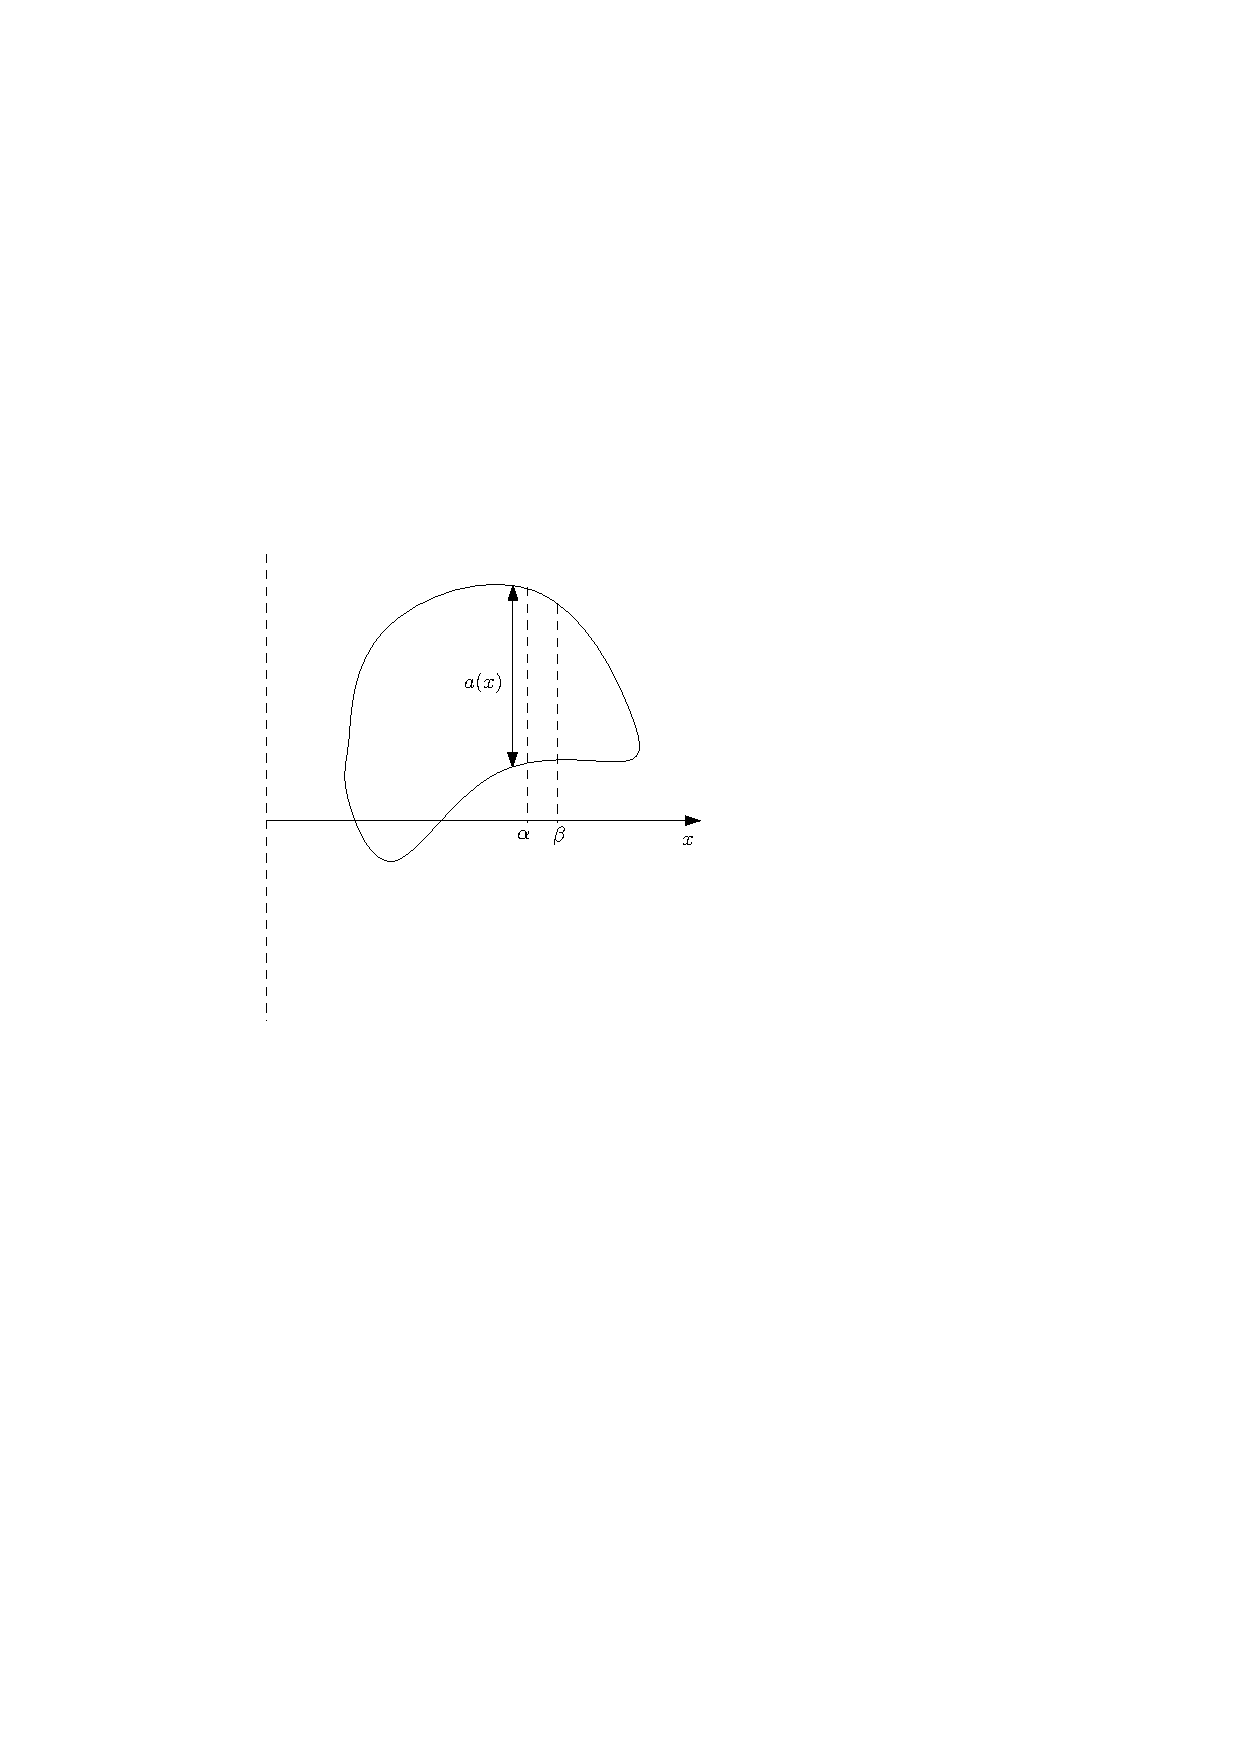
\includegraphics[scale=0.85]{moment}
  
  Докажем, что
  \[ 
    N = \int_{x_1}^{x_2} \sigma xa \left( x \right) \, d  x 
  \]
  где $a \left( x \right)$~--- длина ``сечения''
  фигуры, $\sigma$~--- поверхностная
  плотность
  
  Пусть $\Delta = [ \alpha, \beta ] \subset [ x_1, x_2 ]$~--- промежуток на оси $x$, 
  $\Phi ( \Delta )$~--- момент такой ``полоски''.
  
  Будем считать статический момент аддитивным по определению. Ещё мы умеем считать момент точки: он равен $m_i x_i$.
  Чтобы воспользоваться тестом~\ref{stat:denstest3} докажем, что (то, что они все положительные, очевидно)
  \[ 
    \left( \min_{\Delta} a \left( x \right) \right)  \left( \min_{\Delta} x
    \sigma \right)  \left| \Delta \right| \leqslant \Phi \left( \Delta
    \right) \leqslant \left( \max_{\Delta} a \left( x \right) \right)  \left(
    \max_{\Delta} x \sigma \right) \left| \Delta \right| 
   \]
  \begin{align*}
    & \left( \min_{\Delta} a \left( x \right) \right)  \left| \Delta
    \right| = \left| \Delta \right| a_{\min} = S_1 \text{~---вписанная площадь полоски}\\
    & \left( \max_{\Delta} a \left( x \right) \right)  \left| \Delta
    \right| = \left| \Delta \right| a_{\max} = S_2 \text{~---описанная площадь полоски}\\
    & \left( \min_{\Delta} x \right) = \alpha \\
    & \left(\max_{\Delta} x \right) = \beta 
  \end{align*}
  
  Тогда нижний предел~--- это если бы мы
  сгребли всю массу с $S_1$ и поместили в
  ближний к оси край и посчитали момент
  всего этого. Видно, что момент полоски на
  самом деле больше: и масса оценена снизу,
  и есть хотя бы одна точка с ненулевой
  массой дальше от оси чем $\alpha$.
  Аналогичные рассуждения применимы про
  оценку сверху.
  
  Все условия теста \ref{stat:denstest3} выполнены,
  значит
  \[ 
    N_{\Delta} = \Phi \left( \Delta \right) = \int_{\Delta} a(x) x \sigma \, d  x 
   \]
\end{exmp}

\begin{exmp}
  Работа, которую нужно затратить на
  возведение пирамиды.
  
  \medskip
  
  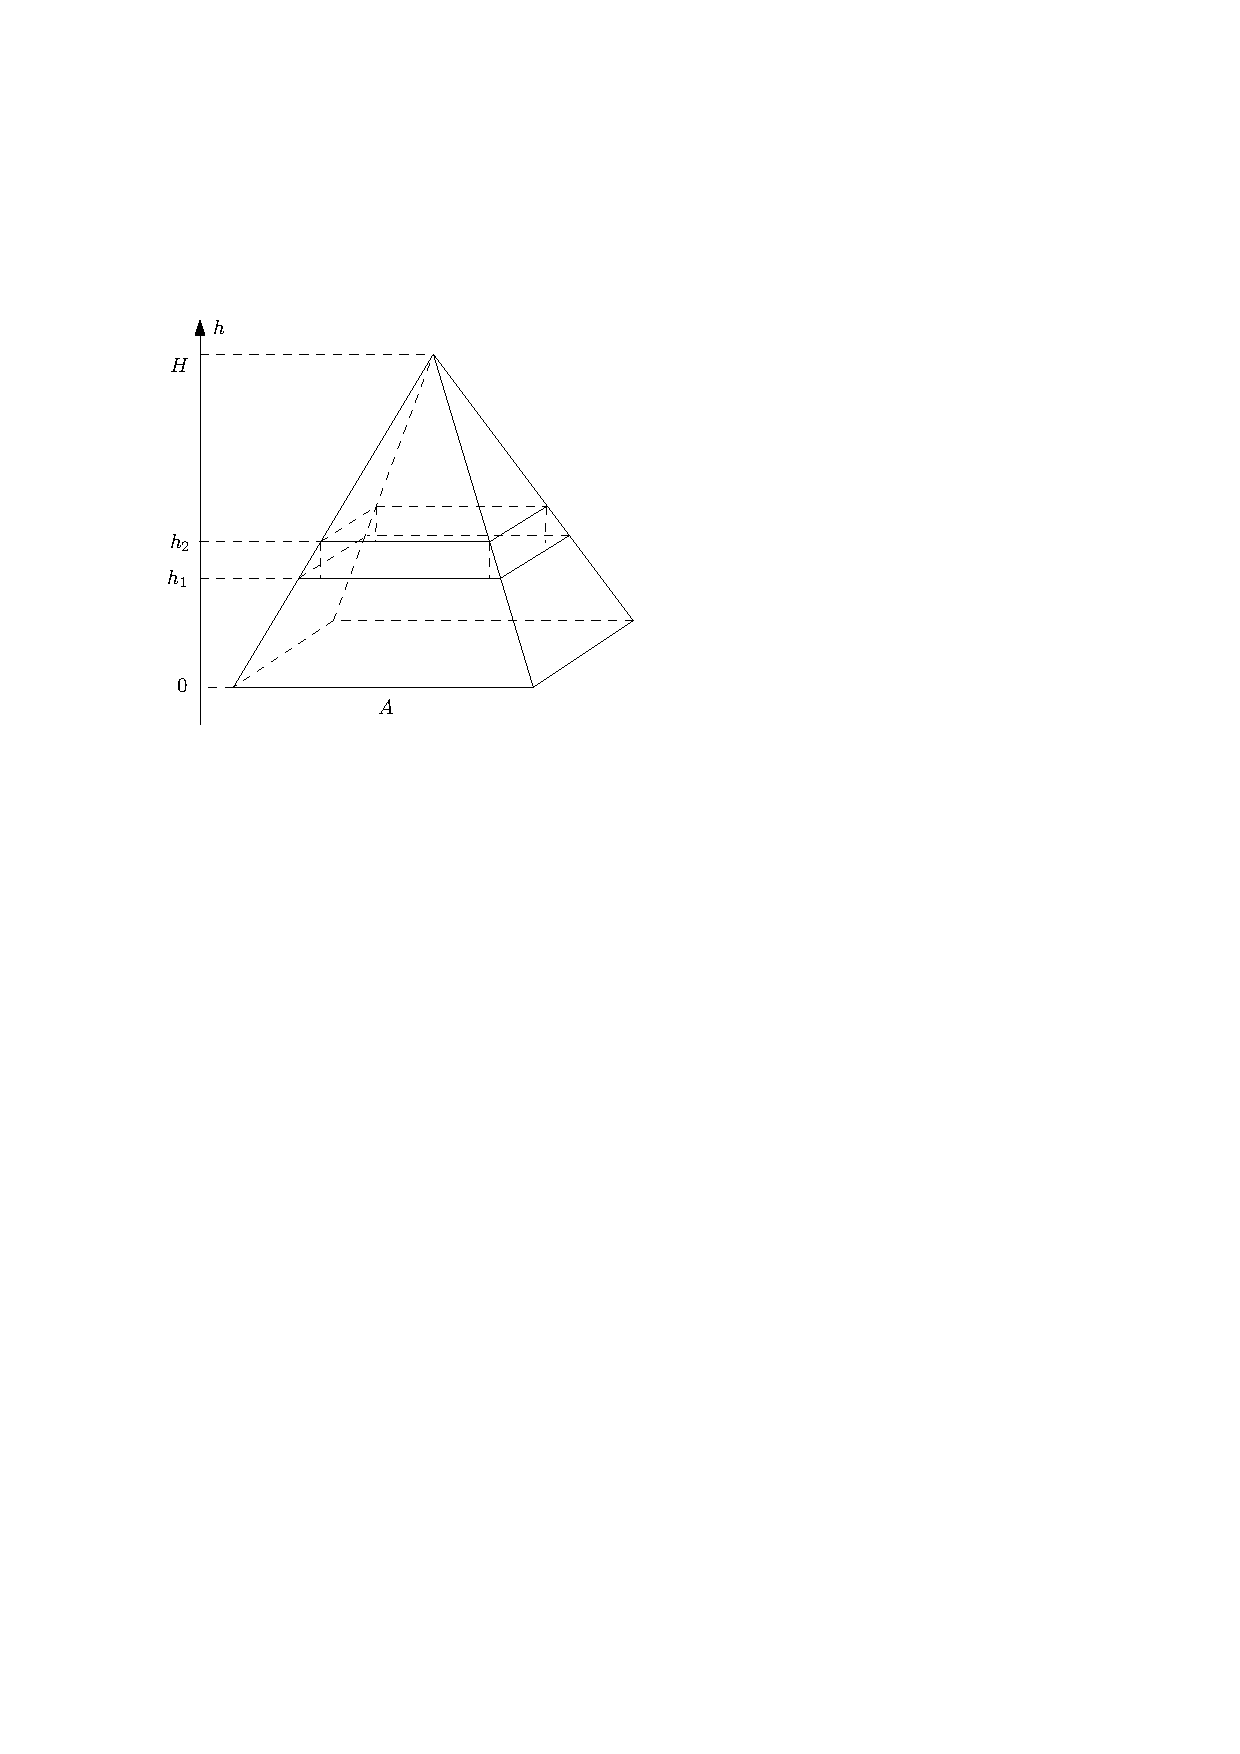
\includegraphics[scale=0.85]{pir}
  
  Пусть $\Delta = \left[ h_1, h_2 \right] \subset \left[ 0 ; H \right]$~--- промежуток на оси высот, 
  $\Phi \left(\Delta \right)$~--- работа которую нужно
  затратить чтобы поднять слой толщины $\left| \Delta \right|$ на нужную высоту, $a \left( h \right)$~---
  сторона пирамиды в зависимости от высоты (она правильная и с квадратом в  основании).
  
  Чтобы получить функцию плотности,
  посмотрим сначала, что происходит с
  блоком в форме параллелепипеда со
  стороной основания $a$. Если поднять его на
  высоту $h$ то работа, затрачена на это
  --- $mgh = \rho a \left( h \right)^2 hg$.
  
  Теперь, давайте докажем, что
  \[ 
    \Phi \left( \Delta \right) = \int_{\Delta} a \left( h \right)^2 hg \, d h 
  \]
  
  
  Будем пользоваться условием теста
  \ref{stat:denstest3}
  \[ \left( \min_{\Delta} a \left( x \right)^2 \right)  \left( \min_{\Delta}
     x \rho \right)  \left| \Delta \right| \leqslant \Phi \left( \Delta
    \right) \leqslant \left( \max_{\Delta} a \left( x \right)^2 \right) 
    \left( \max_{\Delta} x \rho \right) \left| \Delta \right| 
  \]
  
  
  Как видно, от предыдущего примера
  отличается только степенью при $a \left( x
  \right)$. Доказательство здесь почти такое
  же, разве что вместо площадей~--- объёмы.
  
  У нормальной пирамиды $a \left( h \right) = A \frac{H - h}{H}$. Тогда
  \[ 
    A = \int_0^H A^2  \left( 1 - \frac{h}{H} \right)^2 h \rho \, d \, x =
    \rho \frac{A^2}{H^2}  \left( \frac{H^4}{2} - \frac{2 H^4}{3} +
    \frac{H^4}{4} \right) = \frac{1}{12} \rho A^2 H^2 
  \]
  
\end{exmp}

\paragraph{Путь и кривая}
\begin{defn}\label{defn:path}
  Пусть $\gamma \colon [a;b] \to \R^2$, $\gamma$~--- непрерывна (в многомерном смысле). 
  Тогда $\gamma$~--- \emph{путь} на плоскости. Путь~--- отображение.
\end{defn}
\begin{defn}\label{defn:pathcarr}
  Множество $\Gamma = \gamma([a;b])$~--- носитель пути. $\gamma$ в таком случае называется \emph{параметризацией}
  $\Gamma$. 
\end{defn}

\begin{defn}\label{defn:simppath}
  Путь называется \emph{простым}, если отображение $\gamma$~--- биекция.
\end{defn}

\begin{defn}\label{defn:curve}
  Носитель простого пути называется \emph{кривой} \cite{zorich} в $\R^2$ (ну или в $\R^3$, путь туда был).
\end{defn}

\begin{rem*}
  Полезно заметить, что у одной и той же кривой есть много параметризаций. 
\end{rem*}

\begin{exmp*}
  \begin{align*}
    \gamma_1 : 
    \begin{cases}
      x(t) = t \\
      y(t) = t
    \end{cases}, t \in (0;+\infty) & &
    \gamma_2 :
    \begin{cases}
      x(t) = e^{t^3-547} \\
      y(t) = e^{t^3-547} \\
    \end{cases}, t \in \R
  \end{align*}
\end{exmp*}

\begin{defn}\label{defn:curvelen}
  Пусть $\Gamma$~--- кривая, $\gamma\colon [a;b] \to \R^2$~--- её параметризация.

  \begin{tabular}[h]{ll}
    $\tau: a = t_0 < t_1 < \dotsb < t_n = b$ & разбиение отрезка $[a;b]$ \\
    $A_i = \gamma(t_i)$, $p(\tau) = A_1\dotso A_n$ & ломанная, вписанная кривую \\
    $\displaystyle \ell(p(\tau)) = \sum_{i=0}^{n-1} |A_iA_{i+1}|$ & длина ломанной
  \end{tabular}
  
  Тогда длина пути определяется так:\footnote{Длину кривой мы видимо считаем по определению равной длине пути}
  \[
    l(\gamma) := \sup_\tau \ell(p(\tau))
  \]
  При таком определении аддитивность вроде как очевидна ($\sup (\ell_1+\ell_2) = \sup \ell_1 + \sup \ell_2$).
\end{defn}

\paragraph{Вычисление длины гладкого пути}
\begin{thrm}
  Пусть $\Gamma$~--- кривая с гладкой параметризацией $\gamma \colon [a;b]\to R$, $\gamma(t) = (x(t),y(t))$,
  $\gamma \in C^1([a;b])$.
  Тогда длину пути можно найти так: 
  \[
    \ell = \int_a^b \sqrt{x'^2+y'^2} = \int_a^b |\gamma'| \quad \forall\,\gamma
  \]
\end{thrm}
\begin{ittproof}
  Пусть $[\alpha, \beta]=\Delta \subset [a;b]$, $\Phi(\Delta) = \ell(\gamma\big|_\Delta)$. К тому же, как заметили
  выше, $\Phi$~--- аддитивна. Докажем, что $\gamma'$~--- её плотность.

  Будем пытаться свести всё к тесту~\ref{stat:denstest1}. Пусть 
  \begin{align*}
    & m(\Delta) = \sqrt{\left( \min_\Delta |x'(t)| \right)^2 + \left( \min_\Delta |y'(t)| \right)^2}\\
    & M(\Delta) = \sqrt{\left( \max_\Delta |x'(t)| \right)^2 + \left( \max_\Delta |y'(t)| \right)^2}
  \end{align*}
  Условия теста:
  \begin{enumerate}
    \item $m(\Delta) \leqslant \dfrac{\ell(\Gamma_\Delta)}{|[\alpha;\beta]|} \leqslant M(\Delta)$ \\
      Посмотрим на кусочек кривой, который $\gamma(\Delta)$. Разобьём отрезок $[\alpha;\beta]$ 
      и приблизим кривую ломаной, как это делали в~\ref{defn:curvelen}. Тогда по теореме Лагранжа 
      длину звена ломаной можно записать так
      \begin{align*}
        & |A_i A_{i+1}| = \sqrt{|\Delta x_i|^2 + |\Delta y|^2}  = |\Delta t_i|\sqrt{(x'(\xi_1))^2 + (y'(\xi_2))^2}\\
        & |\Delta x_i| = |x'(\xi_1) \Delta t_i|, \; \xi_1 \in [t_i; t_{i+1}] \subset \Delta\\
        & |\Delta y_i| = |y'(\xi_2) \Delta t_i|, \; \xi_2 \in [t_i; t_{i+1}] \subset \Delta
      \end{align*}
      Отсюда понятно как ограничить длину звена 
      \[
        m(\Delta)|\Delta t_i| \leqslant |A_i A_{i+1}| \leqslant M(\Delta) |\Delta t_i|
      \]
      Сложим все такие неравенства:
      \[
        m(\Delta)|\Delta| \leqslant \ell(p) \leqslant M(\Delta) |\Delta|
      \]
      Перейдём к супремуму:
      \[
        m(\Delta) |\Delta| \leqslant \Phi(\Delta) \leqslant M(\Delta) |\Delta|
      \]
    \item очевидно из определения $m, M$
    \item из теоремы Вейерштрасса 
      \[
        \exists\, t^m , t_m \in \Delta \colon |x'(t_m)| = \min_\Delta |x'(t)|, |x'(t^m)| = \max_\Delta |x'(t)|
      \]
      Тогда при $\alpha,\beta \to t$ точки где достигаются экстремальные значения
      $t_m, t^m \to x$ и по непрерывности $x(t)$ $x(t_m),x(t^m) \to x(t)$.
      То же самое рассуждение и для $y(t)$ применимо. А тогда $|m(\Delta)-M(\Delta)|\to0$.
  \end{enumerate}
  Все условия выполнены, значит
  \[
    \Phi(\Delta) = \int_\Delta |\gamma'| \Rightarrow \ell(\gamma)  = \int_{a}^{b} |\gamma'(t)|\,dt
  \]
\end{ittproof}

\paragraph{Геометрический смысл обратных тригонометрических функций }
\def\arch{\ensuremath \operatorname{arch}}
\begin{figure}[t]
  \centering
  \begin{minipage}{0.48\linewidth}
    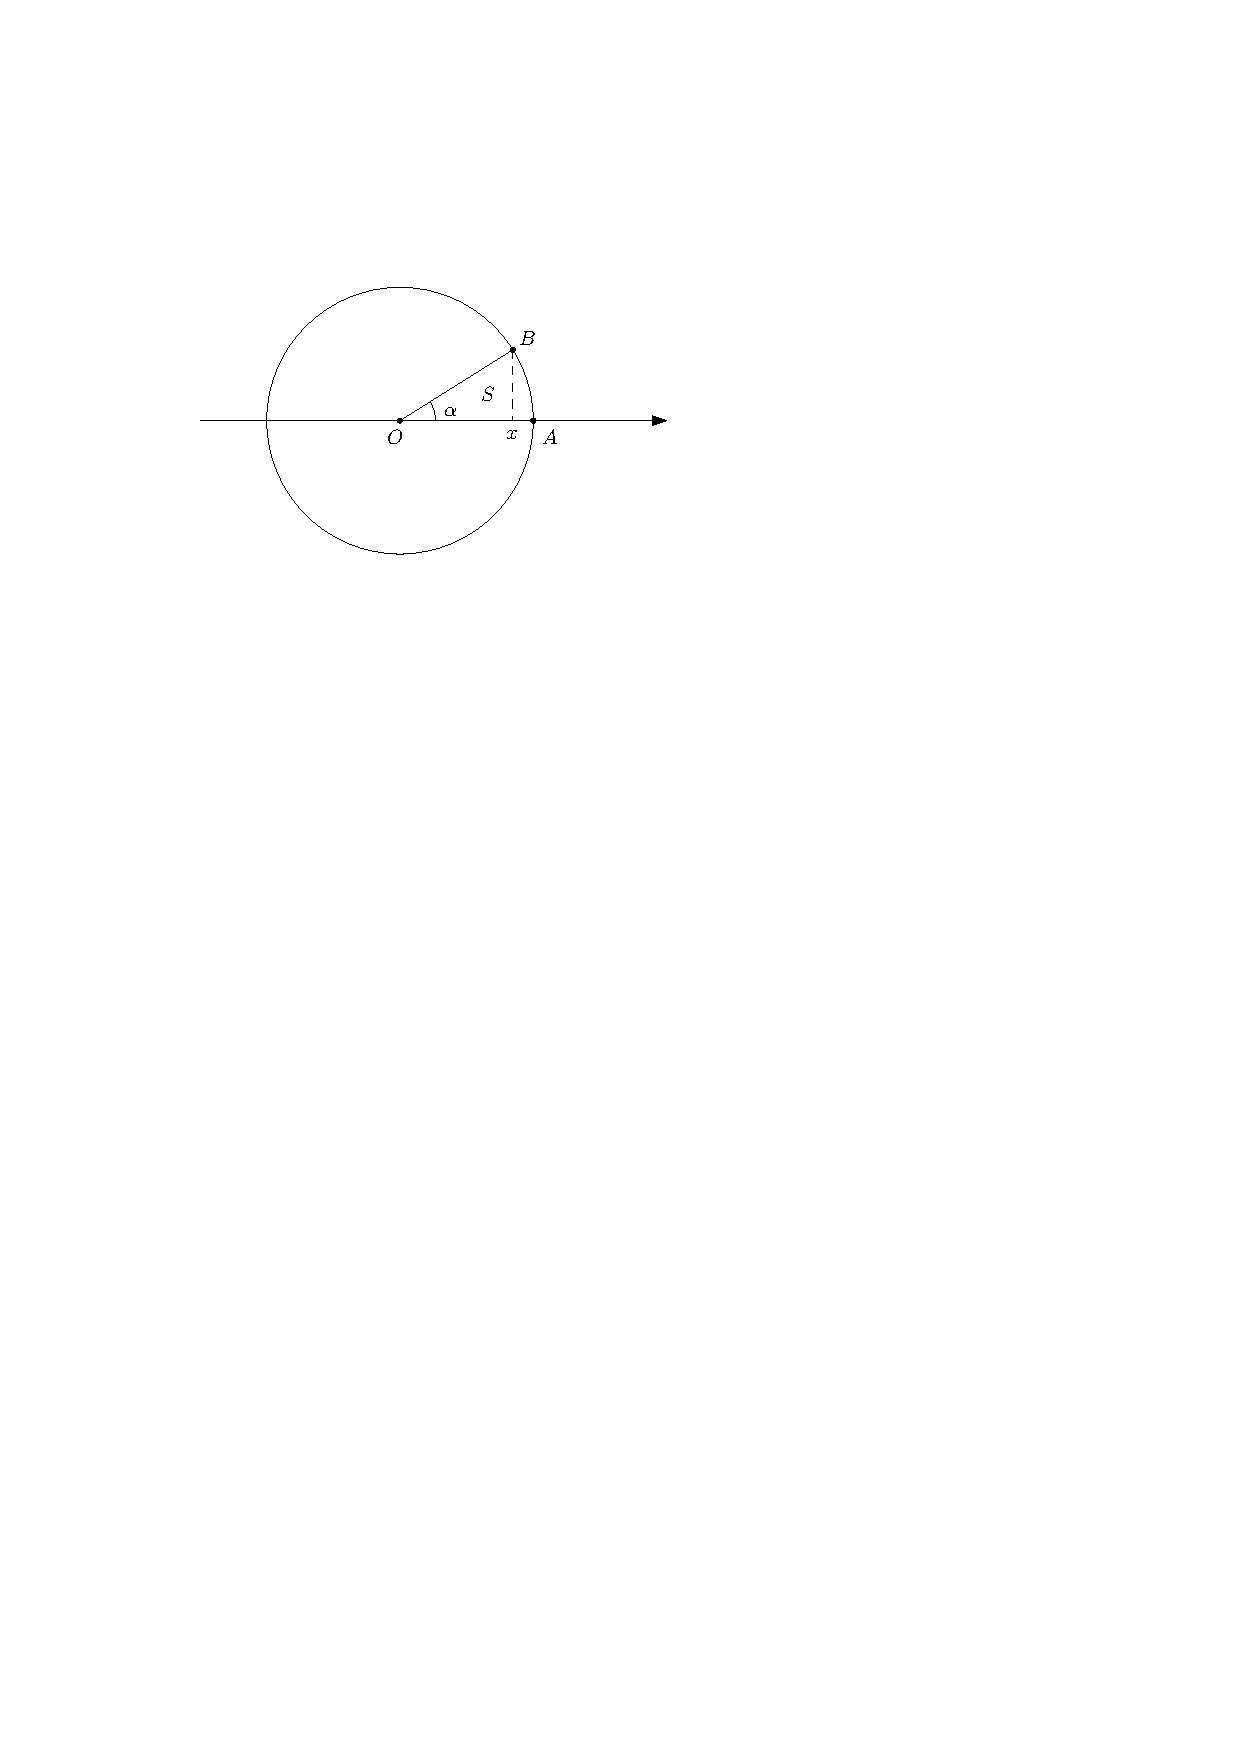
\includegraphics[scale=0.85]{acosgeomsense}~
  \end{minipage}
  \hfill
  \begin{minipage}{0.48\linewidth}
    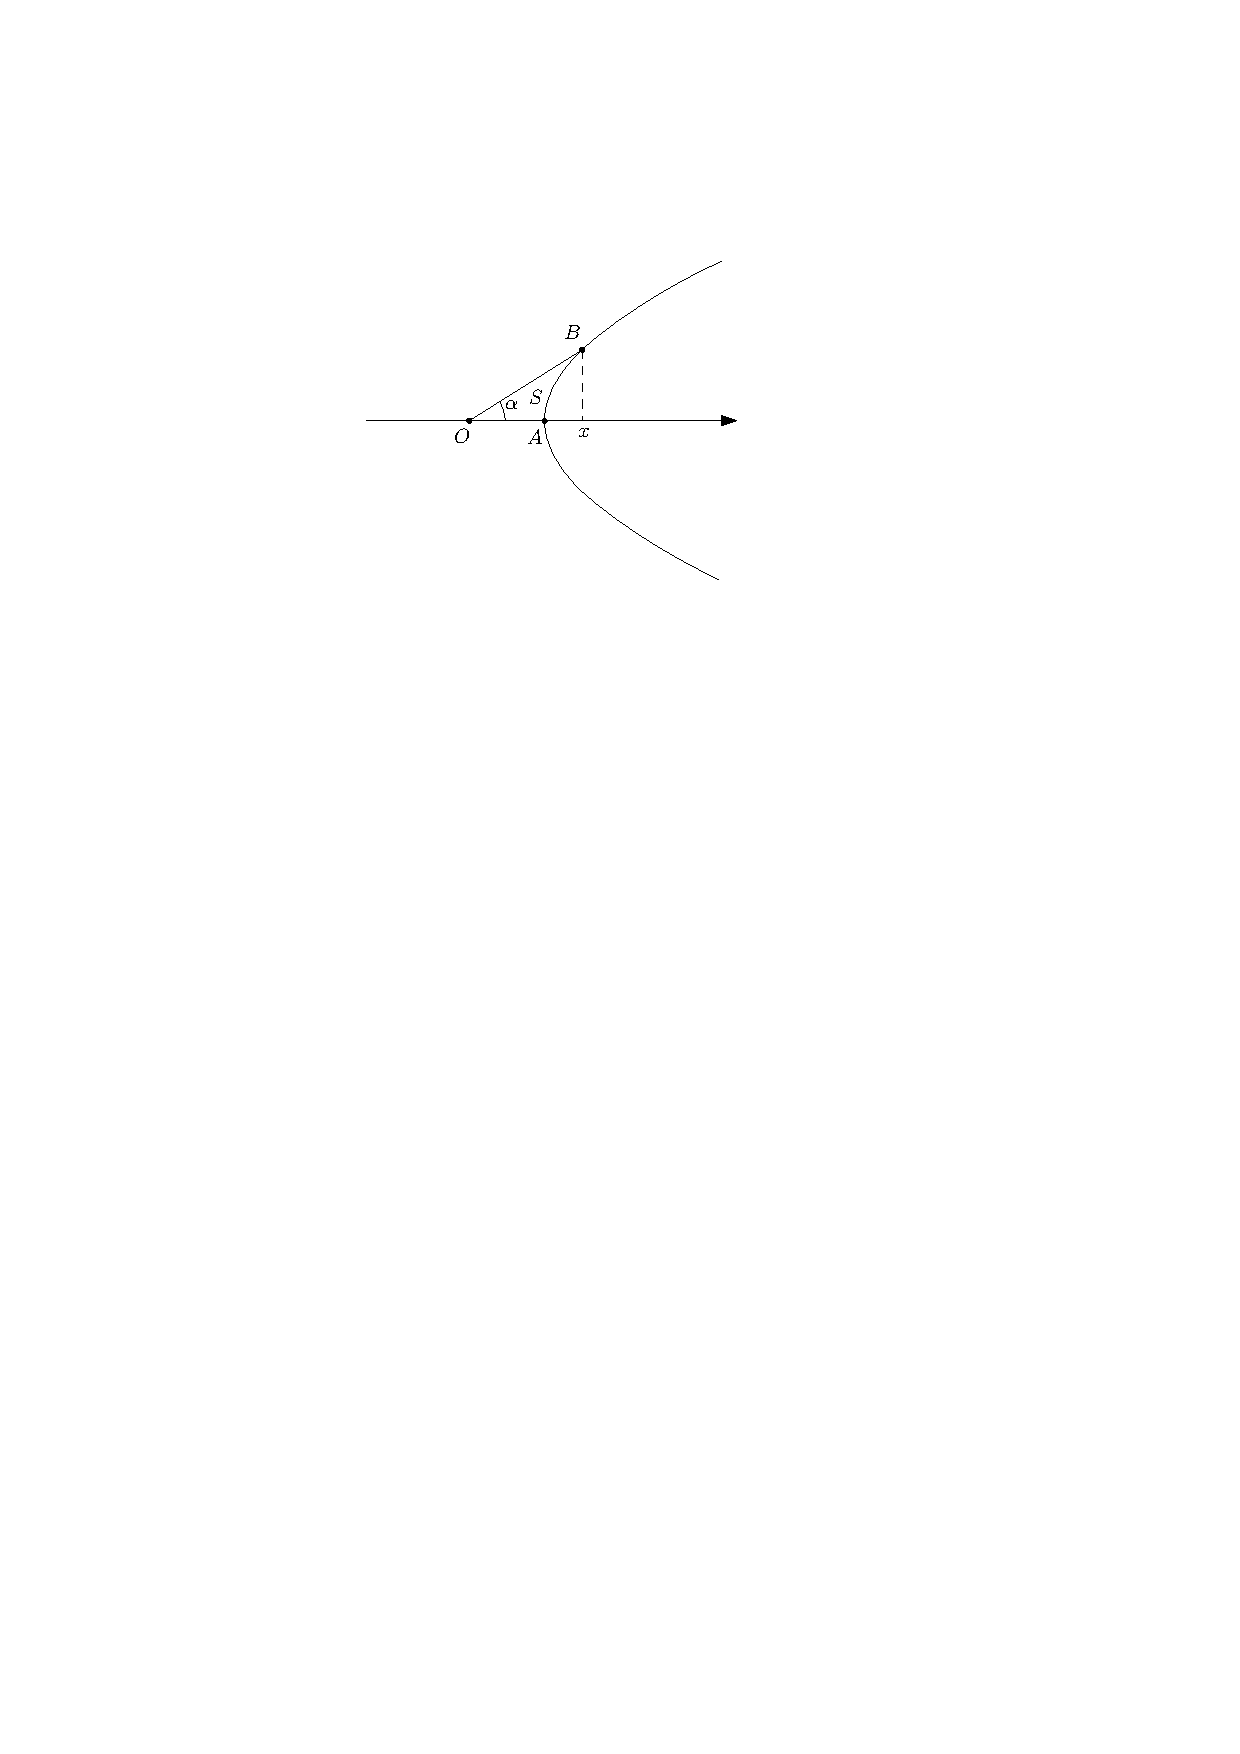
\includegraphics[scale=0.85]{achgeomsense}
  \end{minipage}
  \caption{Иллюстрация к геометрическому смыслу}
  \label{fig:acgeomsense}
\end{figure}
см. Рис.~\ref{fig:acgeomsense} 
\begin{align}
  &x = \cos t \Rightarrow t = \arccos x = \frac{1}{2}S_{AOB} \\
  &x = \ch t \Rightarrow t = \arch x = 2S_{AOB}
\end{align}
\end{document}


\chapter{Несобственные интегралы}
\documentclass[12pt]{../../notes}
\usepackage{silence}
\WarningFilter{latex}{Reference}
\graphicspath{{../../img/}}

\begin{document}
\paragraph{Общие свойства несобственного интеграла}

\begin{defn}\label{defn:impint}
  Пусть $f \in C\big([a;b)\big)$, $b\in \overline{\R}$. 
    Тогда 
    \[
      \int_a^{\to b} f := \lim_{t \to b-0} \int_a^t f
    \]
  Аналогичным образом можно поступить и для нижнего предела (или обоих сразу)
\end{defn}

\begin{defn}\label{defn:intconv}
  $\displaystyle \int_a^{\to b}$ называется \emph{сходящимся}, если он существует и конечен.
\end{defn}
Свойства несобственного интеграла:
\begin{enumerate}
  \item $f \in C \big([a;b]\big)$, $a, b \in \R$. Тогда 
    \[
      \int_a^{\to b} f = \int_{\to a}^b f = \int_a^b f
    \]
  \item $f \in C \big([a;b)\big)$, $c \in (a;b)$ Тогда 
    \[
      \int_a^{\to b} f = \int_a^c f + \int_c^{\to b} f
    \]
    Второе слагаемое ещё называют остатком.
    \[
      \int_a^{\to b} f \text{ сходится } \Leftrightarrow \int_c^{\to b} f \text{ сходится }
    \]
  \item $f \in C \big([a;b)\big)$, $c \in (a;b)$. Тогда 
    \[
      \int_a^{\to b} f \conv \Rightarrow \int_c^{\to b} f \xrightarrow[c\to b]{} 0
    \]
  \item $f,g \in C \big([a;b)\big)$. Тогда 
    \[
      \int_a^{\to b} (f+g) = \int_a^{\to b} f + \int_a^{\to b} g
    \]
  \item $f \in C \big([a;b)\big)$, $c\in \R$
    \[
      \int_a^{\to b} c f = f \int_a^{\to b} f 
    \]
\end{enumerate}
\begin{exmp}
  \[
    \int_1^{+\infty} = \begin{cases} \frac{1}{p-1}, & p > 1 \\ +\infty, & p \leqslant 1 \end{cases}
  \]
\end{exmp}

\paragraph{Признак Больцано-Коши сходимости интеграла}

Этот кусочек не сильно нужен, так что он будет {\footnotesize таким шрифтом}
\begin{footnotesize}

\begin{defn}
  Пусть $f: I \to \R$, $c\in \overline{\R}$~--- точка сгущения. Тогда $f$ сходится в себе при $x\to c$
  $\Leftrightarrow$
  \[
    \forall\, \varepsilon > 0 \;\: \exists\, V(c) \colon \; \forall\,x', x'' \in \overset{\circ} V 
    \;\: |f(x') - f(x'')| < \varepsilon
  \]
\end{defn}

\begin{thrm}[Теорема Больцано-Коши для функций]\label{thrm:bkfun}
  $f$ сходится в себе при $x\to c$ $\Leftrightarrow$ $\exists\,\lim_c f = M \in \R$.
\end{thrm}
\begin{ittproof}
  \begin{description}
    \item[\circlearound{$\Leftarrow$}]  Рассмотрим произвольный $\varepsilon > 0$. Тогда из условия конечности
      предела $\lim_c f$
      \[
        \exists\, V(c) \colon \forall\, x \in V \;\: | f(x) - M | < \varepsilon/2
      \]
      Тогда для $x',x'' \in V(c)$ 
      \[
        |x' - x''| = |(x' - M) - (x''- M)| \leqslant |x' - M| + |x'' - M| < \varepsilon 
      \]
    \item[\circlearound{$\Rightarrow$}] Будем доказывать через аналогичную теорему для последовательностей
      и определение предела по Гейне. Рассмотрим произвольную $(x_n)\colon x_n \to c, x_n \neq c$, 
      произвольный $\varepsilon > 0$.
      Из условия равномерной сходимости
      \[
        \exists\, V(c) \colon \forall\, x', x'' \in \overset{\circ}{V} |f(x') - f(x'')| < \varepsilon
      \]
      $x_n \to c \Rightarrow$
      \[
        \exists\, N \colon \forall\, m,n > N \;\: x_m, x_n \in \overset{\circ}{V}
      \]
      Ну тогда $x' = x_n, x'' = x_m$ и по определению равномерной сходимости последовательностей 
      $y_n = f(x_n)$~--- фундаментальная. А значит, по теореме Больцано-Коши для последовательностей
      $\exists\, \lim y_n = L \in \R$.

      Хорошо, мы получили, что для каждой последовательности $(x_n)$ существует какой-то конечный предел 
      последовательности $y_n = f(x_n)$. Для определения по Гейне необходимо, чтобы они все были равны.

      Хорошо, пусть
      \begin{align*}
        &x_n' \to c  & y_n' = f(x_n') \to L' \\
        &x_n'' \to c  & y_n'' = f(x_n'') \to L''
      \end{align*}
      Тогда $\sphericalangle$ $z_n := (x_1', x_1'', x_2', x_2'', \dotsc)$. Она тоже $\to c$, 
      значит $\exists\, M \in \R\colon f(z_n) \to M$. 
      Но тогда у её подпоследовательностей разные пределы, что странно. 
  \end{description}
\end{ittproof}
\end{footnotesize}

\begin{thrm}\label{thrm:bkconvint}
  Пусть $f \in C\big([a;b)\big)$, $b\in \overline{\R}$. Тогда
  \[
    \int_a^b f \conv \Leftrightarrow \forall\, \varepsilon > 0 \;\: \exists\, V(b) 
    \colon \forall\,t',t''\in \overset{\circ}{V} \;\: \left|\int_{t'}^{t''} f\right| < \varepsilon
  \]
\end{thrm}

\paragraph{Свойства несобственного интеграла от положительных функций}
Пусть $f\in C\big([a;b)\big)$, $f \geqslant 0$, $F'=f$.
\begin{enumerate}
    \setcounter{enumi}{-1}
  \item $\displaystyle \int_a^{\to b} f \conv \Leftrightarrow F(x) \leqslant M \; \forall\, x$ 
  \item\label{stat:intcmp} Признак сравнения интегралов.\\
    Пусть $0 \leqslant f(x) \leqslant g(x)$. Тогда 
    \begin{align*}
      \int_a^{\to b} g \conv \Rightarrow \int_a^{\to b} f \conv \\ 
      \int_a^{\to b} f \noconv \Rightarrow \int_a^{\to b} g \noconv 
    \end{align*}
    Хватит и выполнения неравенства на $[c;b)$, $c \in (a;b)$, всё равно нужен только остаток.
    \item\label{stat:intcmplim} Второй признак сравнения.\\
      Пусть $\displaystyle \exists\, \lim_{t \to b-0} \frac{f(t)}{g(t)} = L$
      Тогда:
      \begin{enumerate}
        \item $\displaystyle L < +\infty 
          \Rightarrow \left(  \int_a^{\to b} g \conv \Rightarrow \int_a^{\to b} f \conv \right)$
        \item $\displaystyle L > 0 
          \Rightarrow \left(  \int_a^{\to b} f \conv \Rightarrow \int_a^{\to b} g \conv \right)$
      \end{enumerate}
      В частности, из эквивалентности следует одинаковый характер сходимости
\end{enumerate}
Попутно в этом же месте нормально определяли всякую тригонометрию, но, кажется, это не нужно в билете.

\paragraph{Абсолютная и условная сходимость интеграла}
\begin{defn}\label{defn:absintconv} 
  Пусть $\dint_a^{\to b}$~--- сходится. Тогда говорят, что он абсолютно сходится, 
  если $\dint_a^{\to b} |f| < + \infty$. В противном случае говорят, что интеграл сходится условно.
\end{defn}

\begin{thrm}\label{thrm:absconv2conv}
  Если интеграл абсолютно сходится, то он сходится.
\end{thrm}
\begin{ittproof}
  $\sphericalangle\,g  = |f| - f$. 
  Тогда $-|f| \leqslant f \leqslant |f| \Rightarrow 0 \leqslant g \leqslant 2|f|$. Теперь всё положительно
  и можно пользоваться признаками сравнения.
  Ещё можно воспользоваться признаком Больцано-Коши~\ref{thrm:bkconvint}~\cite{zorich}.
\end{ittproof}


\paragraph{Признаки Дирихле и Абеля}
\begin{thrm}[Признак сходимости Дирихле]\label{thrm:imprdirconv}
  Пусть $f,g \in C^1\big([a;b)\big)$\footnote{Вообще, хватило бы и просто непрерывности, 
  но для этого нужно доказывать ещё сколько-то интегральных неравенств о среднем 
  такого сорта : 
  \[
    \exists\, \xi \in [a;b]\colon \int_a^b (fg) = g(b)\int_a^\xi f + g(a) \int_\xi^b f
    \text{ \hspace{1cm} (см.~\cite[стр.~469]{zorich}) } \] } и 
  \begin{enumerate}
    \item $|f(x)|$\footnote{Вообще, мы формулировали это без модуля, 
      но для непрерывных функций эти условия эквивалентны} $\searrow 0$ при $x \to b-0$
    \item $\exists\,M: \left|\int_a^t g\right| \leqslant M \;\, \forall\, t $
  \end{enumerate}
  Тогда $\dint_a^{\to b} fg$~--- сходится
\end{thrm}
\begin{thrm}[Признак сходимости Абеля]\label{thrm:imprabelconv}
  Пусть $f,g \in C^1\big([a;b)\big)$ и 
    \begin{enumerate}
      \item $f(x)$ монотонна и ограничена
      \item $\int\limits_a^{\to b} g$ сходится
    \end{enumerate}
  Тогда $\dint_a^{\to b} fg$~--- сходится
\end{thrm}
\begin{ittproof}
  Доказывать всё надо через признак Больцано-Коши~\ref{thrm:bkconvint}. Сначала проинтегрировать по частям,
  а потом долго оценивать и доказывать что всё $\to 0$.
\end{ittproof}


\end{document}


\chapter{Числовые ряды}
\documentclass[12pt]{../../notes}
\usepackage{silence}
\WarningFilter{latex}{Reference}
\graphicspath{{../../img/}}

\begin{document}
\paragraph{Числовые ряды и примеры оных}
\begin{defn}\label{defn:numseries}
  Пусть $(a_n)_{n=1}^\infty,\; a_n \in \R$~--- числовая последовательность.
  Тогда рядом можно назвать последовательность и желание её просуммировать\smiley.
  \begin{itemize}
    \item Элементы последовательности $(a_n)$~--- члены ряда.
    \item $S_n = \dsum_{k=1}^m a_k $~--- частичная сумма последовательности $(a_n)$
    \item $r_m = \dsum_{k=m+1}^\infty a_k$~---  остаток ряда.
    \item $S = \dsum_{k=1}^\infty a_k := \lim_{n \to \infty} S_n$~--- сумма ряда.
  \end{itemize} 
  В принципе, ряд можно попробовать формализовать как упорядоченную пару $\big((a_n),(S_n)\big)$.
  Или просто называть рядом некий цельный символ $\sum_{n=1}^\infty a_n$.
\end{defn}

\begin{defn}\label{defn:num}
  Ряд называется \emph{сходящимся} когда предел частичных сумм существует и конечен и 
  \emph{расходящимся} во всех остальных случаях.
\end{defn}

\begin{exmp}
  \[
    \sum_{k=1}^{\infty} \frac{1}{k(k+1)} = \frac{1}{1\cdot2} + \frac{1}{2\cdot3} + \frac{1}{3\cdot4} +\dotsb
  \]
  Посмотрим на член ряда:
  \[
    \frac{1}{k(k+1)} = \frac{1}{k} - \frac{1}{k+1}
  \]
  Перепишем ряд:
  \[
    \sum_{k=1}^{n} = \left( 1 - \frac{1}{2} \right) + \left( \frac{1}{2} - \frac{1}{3} \right) + \dotsb 
    + \left( \frac{1}{n} - \frac{1}{n+1} \right) = 1 - \frac{1}{n+1}
  \]
  Оно магически свернулось. Теперь: 
  \[
    S = \lim_{n\to \infty} \left( 1 - \frac{1}{n+1} \right) = 1
  \]
\end{exmp}
\begin{exmp}\label{exmp:geomseries}
  \[
    \begin{cases}
      \dsum_{n=0}^\infty q^n = \frac{1}{1-n}, & |q| < 1 \\
      \text{ ряд расходится },  & |q| \geqslant 1 \\
    \end{cases}
  \]
\end{exmp}

\paragraph{Общие свойства числовых рядов}
\begin{enumerate}
  \item $\dsum_{k=1}^\infty a_k \conv \Rightarrow a_k \xrightarrow[k\to \infty]{} 0$
  \item ряд сходится $\Leftrightarrow$ его остаток сходится.
  \item $\dsum_{k=1}^\infty(a_k + b_k) = \dsum_{k=1}^\infty a_k + \dsum_{k=1}^\infty b_k $
     (если любые  2 ряда сходятся, то сходится и третий).
   \item $\forall c\in \R\; \dsum_{k=1}^\infty c\,a_k = c \dsum_{k=1}^\infty a_k$
     (характер сходимости у рядов одинаковый)
   \item $\dsum_{k=1}^\infty a_k \conv 
     \Leftrightarrow r_m \! = \!\!\dsum_{k=m+1}^\infty a_k \xrightarrow[m\to\infty]{} 0$
\end{enumerate}
\begin{stat}[Критерий сходимости Больцано-Коши]\label{stat:bkseriesconv}
  \[
    \sum_{k=1}^\infty a_k \conv \Leftrightarrow \forall\,\varepsilon > 0 \; \exists\, N: \forall\, n > N
    \; \forall\, p > 0 \;\: \left| \sum_{k=n+1}^{n+p} a_k \right| < \varepsilon
  \]
\end{stat}

\paragraph{Положительные ряды. Признаки сравнения}
\begin{defn}
  Ряд положителен, если $\forall k \; a_k \geqslant 0$
\end{defn}

\setcounter{thrm}{-1}
\begin{stat}
  Всегда $\exists\, S\in [0; +\infty]$
\end{stat}

\begin{stat}[Первый признак сравнения]\label{stat:cmpseries1}
  Пусть $\forall\, n \; a_n \geqslant b_n \geqslant 0$. Тогда
  \begin{align*}
    \sum_{k=1}^{\infty} a_k \conv   &\Rightarrow \sum_{k=1}^{\infty} b_k \conv \\ 
    \sum_{k=1}^{\infty} a_k \noconv &\Leftarrow \sum_{k=1}^{\infty} b_k \noconv \\ 
  \end{align*}
\end{stat}
\begin{rem*}
 Хватит выполнения неравенства в $V(\infty)$, всё равно сходимость определяют только остатки.
\end{rem*}
\begin{stat}[Второй признак сравнения]\label{stat:cmpseries2}
  Пусть $\forall\, n \; a_n \geqslant 0, b_n > 0$ и также
  \[
    \exists\, \lim_{n\to \infty}\frac{a_n}{b_n} = L \in [0; +\infty]
  \]
  Тогда: 
  \begin{align*}
    L <+\infty \Rightarrow \left( \sum_{k=1}^{\infty} b_k \conv \Rightarrow \sum_{k=1}^{\infty} a_k \conv \right)\\
    L > 0 \Rightarrow \left( \sum_{k=1}^{\infty} a_k \conv \Rightarrow \sum_{k=1}^{\infty} b_k \conv \right)\\
  \end{align*}
\end{stat}

\begin{imp}
  При $0 < L < +\infty$ ряды ведут себя одинаково
\end{imp}

\parrange{2}{Признаки Даламбера и Коши}
\begin{thrm}[Признак Даламбера]\label{thrm:dalambconv}
  Пусть $\sum a_n$~--- положительный ряд и 
  \[
    \exists\, D = \lim_{n\to\infty} \frac{a_{n+1}}{a_n}, \; D \in [0;+\infty]
  \]
  Тогда 
  \begin{enumerate}
    \item $D < 1$ $\Rightarrow$ ряд сходится
    \item $D > 1$ $\Rightarrow$ ряд расходится
    \item $D = 1$ $\Rightarrow$ непонятно
  \end{enumerate}
\end{thrm}
\begin{thrm}[Признак Коши]\label{thrm:cauchyconv}
  Пусть $\sum a_n$~--- положительный ряд и 
  \[
    \exists\, C = \lim_{n\to\infty} \sqrt[n]{a_n}, \; C \in [0;+\infty]
  \]
  Тогда 
  \begin{enumerate}
    \item $C < 1$ $\Rightarrow$ ряд сходится
    \item $C > 1$ $\Rightarrow$ ряд расходится
    \item $C = 1$ $\Rightarrow$ непонятно
  \end{enumerate}
\end{thrm}

\begin{rem}
  Оба признака: и Коши и Даламбера~--- основаны на сравнении ряда с геометрической прогресиией~\ref{exmp:geomseries}.
  А сумма геометрической прогрессии сходится, когда её знаменатель $ < 1$. А $q=1$~--- точка в которой
  формула суммы геометрической прогресии не существует. Так что она особенная $\smiley$.
\end{rem}

\begin{rem}
  В качестве примера к 3 пункту обеих теорем годится ряды $\sum \frac{1}{n}$ и $\sum \frac{1}{n^2}$.
  Второй сходится, а первый~--- нет.
\end{rem}

\parrange{2}{Верхний и нижний пределы последовательности}
\begin{defn}\label{defn:limsup}
  Пусть $(x_n)$~--- целочисленная последовательность. Тогда 
  \begin{align*}
    & \underline{\ell} = \llim_{k\to \infty} x_k := \lim_{n\to \infty} \inf_{k\geqslant n} x_k \\
    & \overline{\ell} = \uplim_{k\to \infty} x_k := \lim_{n\to \infty} \sup_{k\geqslant n} x_k
  \end{align*}
  где $\overline{\ell}, \underline{\ell}$~--- верхний и нижний пределы соответственно.
\end{defn}
\begin{rem}
  Можно ещё конечно отдельно упомянуть про случаи с $\pm \infty$, но вроде как все они уже заложены
  в определение предела.
\end{rem}
\begin{rem}
  Верхний и нижний пределы существуют, так как последовательность супремумов/инфимумов монотонна.
\end{rem}

\begin{defn}
  Пусть $(x_n)$~--- целочисленная последовательность, $(x_{n_k})$~--- её подпоследовательность. 
  Тогда $c\in \overline{\R}$:
  \[
    c = \lim_{k\to \infty} x_{n_k} 
  \]
  называется частичным пределом последовательности.
\end{defn}

\begin{thrm}[Теорема о трёх пределах?]
  \[
    \exists\, \lim_{n\to\infty} x_n 
    \Leftrightarrow \llim_{n\to\infty} x_n = \uplim_{n\to\infty} x_n = \lim_{n\to\infty} x_n
  \]
\end{thrm}
\begin{ittproof}
  Следствие теоремы~\ref{thrm:partlimset}
\end{ittproof}

\begin{thrm}[о множестве частичных пределов]\label{thrm:partlimset}
  Пусть $(x_n)$~--- целочисленная последовательность, $\overline{\ell}, \underline{\ell}$~--- её 
  верхний и нижний пределы соответственно. 
  \begin{enumerate}
    \item $c$~--- частичный предел $\Rightarrow \underline{\ell} \leqslant c \leqslant \overline{\ell}$
    \item $\underline{\ell}, \overline{\ell}$ сами являются частичными пределами
  \end{enumerate}
\end{thrm}

\begin{ittproof}
  Пусть 
  \[
    \overline{x_n} = \sup_{i\geqslant n} x_i,\;\underline{x_n} = \inf_{i\geqslant n} x_i,\;
    c = \lim_{k\to \infty} x_{n_k}. 
  \]
  \begin{enumerate}
    \item Из определения $\overline{x_n}$, $\underline{x_n}$ и правила 3 полицейских: 
      \[
        \underline{x_{n_k}} \leqslant x_{n_k} \leqslant \overline{x_{n_k}} \xrightarrow[k\to \infty]{}
        \underline{\ell } \leqslant c \leqslant \overline{\ell}
      \]
      ( тут они ещё не подспоследовательности, но вот брать $n_k$ элемент мы уже умеем ).
    \item Докажем условие для $\overline{\ell}$, для инфимумов там то же самое будет. Из определения предела
      \[
        \forall\, V_1(\overline{\ell}) \;\:\exists\, N \colon \forall n > N \;\: \overline{x_n} \in V_1 
      \]
      К тому же
      \[
        \forall\, n, V_2(\overline{x_n}) \;\: \exists\, k > n \colon x_k \in V_2^- \subset V_2 \text{ 
          ( иначе $\overline{x_n}$ не супремум $\{x_k \mid k\geqslant n\}$). }
      \]
      Тогда $x_k \in V_1 \cup V_2$. А такими объединениями можно собрать любую окрестность.
  \end{enumerate}
\end{ittproof}

\paragraph{Обобщённый признак Коши}
\begin{thrm}\label{thrm:enhcauchyconv}
  Пусть $\sum a_n$~--- положительный ряд и 
  \[
    C = \uplim_{n\to\infty} \sqrt[n]{a_n}, \; C \in [0;+\infty]
  \]
  Тогда 
  \begin{enumerate}
    \item $C < 1$ $\Rightarrow$ ряд сходится
    \item $C > 1$ $\Rightarrow$ ряд расходится
    \item $C = 1$ $\Rightarrow$ непонятно
  \end{enumerate}
\end{thrm}
\begin{rem}
  В отличие от ``обычного'' признака Коши~\ref{thrm:cauchyconv}  тут не стоит вопрос о существовании предела,
  он есть всегда. Этим усиленный признак и лучше.
\end{rem}

\paragraph{Интегральный признак сходимости ряда}
\begin{thrm}
  Пусть $f\in C\big([1;+\infty)\big)$, $f\geqslant 0 $, $f \searrow [1;+\infty)$. 
    Пусть также $a_n  = f(n)$, $n\in \N$.
  Тогда 
  \[
    \sum_{n=1}^{\infty} a_n \conv \Leftrightarrow \int_{1}^{\infty} f \conv
  \]
\end{thrm}

\begin{ittproof}
  Пусть $F(t) = \int_1^t f$, тогда $F \nearrow [1;+\infty)$, $A_n \nearrow$. Значит, все пределы существуют.
    На основании этого немного перепишем условия:
  \begin{align*}
    \int_1^\infty f \conv &\Leftrightarrow \exists\,\sup\limits_{t\geqslant1} F(t) \in \R \\
    \sum_{k=1}^\infty a_k \conv &\Leftrightarrow \exists\,\sup\limits_{n\in\N} A_n \in \R 
  \end{align*}
  \begin{description}
    \item[\circlearound{$\Leftarrow$}] Пусть $k\in \N $, $k \leqslant x \leqslant k+1$. Тогда из
      убывания $f$
    \[
      \int_{k}^{k+1} f(x)\, dx \geqslant \int_{k}^{k+1} f(k+1)\, dx = a_{k+1}
    \]
    Тогда
    \[
      F(n) = \sum_{k=1}^{n-1} \int_{k}^{k+1} f(x)\, dx \geqslant \sum_{k=1}^{n-1} a_{k+1} = A_n - a_1
    \]
    Ну а тогда из ограниченности интеграла следует ограниченность частичных сумм .
  \item[\circlearound{$\Rightarrow$}] 
    \[
      \int_{k}^{k+1} f(x)\, dx \leqslant \int_{k}^{k+1} f(k)\, dx = a_k
    \]
    А дальше аналогично, только ограничиваем частичными суммами интеграл
  \end{description}
\end{ittproof}

\paragraph{Признак Лейбница}
\begin{defn}
  Пусть  $(c_n)$~--- числовая последовательность, $\forall\, n \; c_n > 0$, $c_n \searrow$, $c_n\to 0$
  Тогда $\dsum_{n=0}^\infty (-1)^n c_n$~--- ряд Лейбница (знакопеременный ряд).
\end{defn}
\begin{thrm}\label{thrm:leibseriesconv}
  Про ряд Лейбница можно сказать следующее:
  \begin{enumerate}
    \item Он всегда сходится
    \item $S \in [0; c_0]$
    \item $\forall\,n \; |r_n| \leqslant c_{n+1}$
  \end{enumerate}
\end{thrm}
\begin{ittproof}
  Основная идея доказательства~--- посмотреть на половину ряда (например на чётную) и понять, что 
  её частичные суммы убывают к $0$, а значит и сходятся где-то в $[0;c_0]$. А вторая половина сходится туда же,
  так как члены ряда стремятся к $0$. 

  Наконец, полезный пункт про остаток очевиден, если заметить, что остаток~--- тоже ряд Лейбница.
\end{ittproof}

\paragraph{Признаки Абеля и Дирихле сходимости рядов}
\begin{stat}[Преобразование Абеля]
  Пусть $(a_n), (b_n)$~---  числовые последовательности, $(B_n): B_n = b_1 + \dotsb b_n, \; B_0 = 0$ 
  Тогда 
  \[
    \sum_{k=n+1}^{n+p} a_k b_k = a_{n+p} B_{n+p} - a_{n+1} B_n + \sum_{k=n+1}^{n+p-1} (a_k - a_{k+1}) B_k
  \]
\end{stat}
\begin{itlproof}
  \[
    \begin{split}
      \sum_{k=n+1}^{n+p} a_k b_k & = \sum_{k=n+1}^{n+p} a_k (B_k - B_{k-1} ) \\
                                 & = a_{n+1}B_{n+1} - a_{n+1} B_n + \dotsb + a_{n+p}B_{n+p} - a_{n+p} B_{n+p-1} \\
                                 & = a_{n+p} B_{n+p} - a_{n+1} B_n + \sum_{k=n+1}^{n+p-1} (a_k - a_{k+1}) B_k
    \end{split}
  \]
\end{itlproof}
\begin{rem*}
  По сути, аналог интегрирования по частям, только для для рядов.
\end{rem*}

\begin{thrm}[Признак Дирихле]\label{thrm:serdirsign}
  Пусть $\sum a_k b_k$~--- числовой ряд. Пусть также
  \begin{enumerate}
    \item $a_n \searrow 0 $\footnote{Тут уже трюк с модулем как в~\ref{thrm:imprdirconv} не выйдет}
    \item $\exists\, M : \forall\,n \; |B_n| \leqslant M$
  \end{enumerate}
  Тогда ряд $\sum a_k b_k $ сходится.
\end{thrm}

\begin{thrm}[Признак Абеля]\label{thrm:serabelsign}
  Пусть $\sum a_k b_k$~--- числовой ряд. Пусть также
  \begin{enumerate}
    \item $a_n$ монотонна и ограничена 
    \item $\dsum_{k=1}^\infty b_k \conv$
  \end{enumerate}
  Тогда ряд $\sum a_k b_k $ сходится.
\end{thrm}
\begin{ittproof}
  $a_n$ монотонна и ограничена $\Rightarrow$ имеет конечный предел. Пусть $a_n \to a$. Тогда
  \[
    \sum_{k=1} \infty a_k b_k = \sum_{k=1} \infty (a_k - a) b_k + a\sum_{k=1} \infty b_k 
  \]
  А теперь всё это сходится по признаку Дирихле.~\cite[стр.~309]{ficht2}
\end{ittproof}

\begin{rem*}
  Идеи тут в целом такие же, как и в аналогичных признаках для несобственного интеграла, разве что
  вместо интегрирования по частям~--- преобразование Абеля.
\end{rem*}

\parrange{2}{Группировка и перестановка членов ряда}
\begin{defn}\label{defn:sergroup}
  Пусть $\sum a_k$~--- числовой ряд, $(n_i)$~--- неубывающая последовательность номеров, $n_0=0$. Тогда про ряд 
  \[
    \sum b_k\colon \left( b_k = \mspace{-15mu} \dsum_{n_{k-1} < i \leqslant n_k} \mspace{-15mu} a_i \right)
  \] 
  говорят, что он получен из $\sum a_k$ группировкой слагаемых.
\end{defn}

\begin{thrm}\label{thrm:sergroupprop}
  Пусть $\sum a_k$~--- сходится, а $\sum b_k$ получен из него группировкой слагаемых. Тогда и $\sum b_k$ сходится, 
  причём $\sum a_k = \sum b_k$. Ещё говорят, что ряд обладает сочетательным свойством.
\end{thrm}
\begin{ittproof}
  следствие теоремы о подпоследовательности
\end{ittproof}
\begin{rem*}
  В другую сторону такое свойство неверно, например ряд $(-1)^n$
\end{rem*}

\begin{defn}\label{defn:sercommute}
  Пусть $\sum a_k$~--- числовой ряд, $\pi : \N \to \N$~--- биективное отображение. Тогда про
  ряд 
  \[  
    \sum_{k=1}^\infty b_k \colon b_k = a_{\pi(k)}
  \]
  говорят, что он получен из $\sum a_k$ перестановкой  слагаемых.
\end{defn}
\begin{defn}\label{defn:sercommuteprop}
  Если в рамках предыдущего определения~(\ref{defn:sercommute})
  \[
    \forall\, \pi \; \sum_{n=1}^\infty a_n = \sum_{n=1}^\infty b_n,
  \]
  то говорят, что ряд $\sum a_n$ обладает переместительным свойством.
\end{defn}

\begin{thrm}\label{thrm:sercommutepos}
  Положительные ряды обладают переместительным свойством.
\end{thrm}
\begin{ittproof}
  Пусть ряд $\sum b_n$ получился из положительного ряда $\sum a_n$ перестановкой $\pi : \N \to \N$.
  Посмотрим на частичную сумму $B_n$.
  \[
    B_n = b_1 + \dotsb + b_n = a_{\pi(1)} + \dotsb + a_{\pi(n)} \leqslant \sum_{k=1}^m a_k = A_m, 
  \] где $m = \max\{\pi(k) \mid k\in \{1,\dotsc,n\}\}$ (они все положительно, просто больше членов взяли).
  Таким образом, мы ограничили частичные суммы $\sum b_n$. А значит при переходе к пределам мы получим, что
  $B \leqslant A$.

  Однако $\pi$~--- биекция $\Rightarrow$ $\exists\, \pi^{-1}$. А значит, применяя те же самые рассуждения, 
  мы получим, что $A \leqslant B$. Таким образом, $A=B$.
\end{ittproof}

\begin{thrm}\label{thrm:sercommuteabs}
  Абсолютно сходящиеся ряды обладают переместительным свойством.
\end{thrm}
\begin{defn}
  Пусть $a\in \R$. Тогда 
  \begin{align*}
    a^+ & := \max\{a,0\} \\
    a^- & := \max\{-a,0\} 
  \end{align*}
\end{defn}

\begin{thrm}[Теорема Римана]\label{thrm:sercommuteriman}
  Пусть ряд $\sum a_n$ сходится условно, а $B\in \overline{R}$. Тогда $\exists\, \pi:\N\to\N$ такая, что
  \[
    \sum_{n=1}^\infty a_{\pi(n)} = B
  \]
\end{thrm}
\begin{ittproof}
  Вообще, строгого доказательства не будет, а вот картинка к нестрогому:
  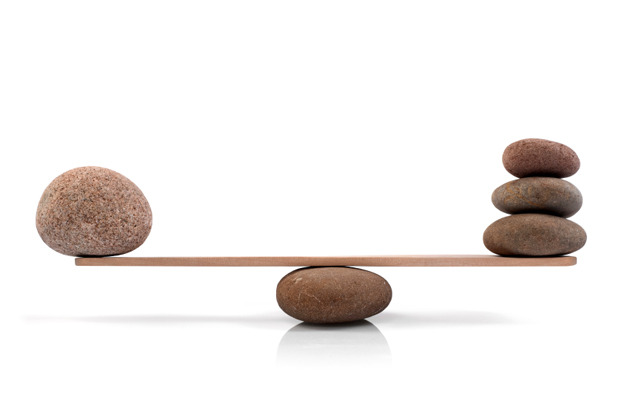
\includegraphics[scale=1]{libra}
  
  Мы можем сначала вынимать из ряда в том порядке, в котором они идут, положительные члены,
  пока не <<перевесим>> нужное значение. Потом вынимаем отрицательные, пока равновесие не сместится обратно.
  Потом снова положительные и так далее. Члены ряда уменьшаются по модулю, разность между <<массами>>
  на весах тоже уменьшается $\to 0$. 
  
  Но вообще, повторюсь, это скорее размахивание перекладиной весов,
  и закидывание оппонента гирьками,  чем доказательство.
\end{ittproof}

Ещё вот подтверждение:
\begin{exmp}
  Пусть $a_k = \frac{(-1)^{k-1}}{k}$, $\sum a_k = A$. Переставим чиселки в такие <<тройки>>:
  \[
    \sum b_k = 1 - \frac{1}{2} - \frac{1}{4} + \frac{1}{3} - \frac{1}{6} -\frac{1}{8} + \dotsb
  \]
  В итоге 
  \[
    \begin{split}
      B_{3n} & = \sum_{k=1}^n \left( \frac{1}{2k-1} - \frac{1}{4k-2} - \frac{1}{4k} \right) \\
      & = \sum_{k=1}^n \left( \frac{1}{4k-2} - \frac{1}{4k} \right) \\ 
      & = \sum_{k=1}^n \frac{1}{2} \left( \frac{1}{2k-1} - \frac{1}{2k} \right)  = \frac{1}{2} A_{2n}
    \end{split}
  \] 
  Таким образом, $B_{3n} \to \frac{1}{2} A$. Все остальное сходится туда же, так как члены ряда $\to 0$
\end{exmp}

\paragraph{Понятие о суммируемом семействе чисел}
Этот кусок вообще какой-то странный\ldots Давайте лучше верить, что ``понятие'' не требует особой строгости
\begin{defn}\label{label:summset}
  Ладно, пусть есть какая-то $(a_i)_{i\in I}$, где $I$~--- множество индексов.
  \begin{enumerate}
    \item Пусть $\forall\,i \; a_i \geqslant 0$, $F \subset I$, $\#F < \infty$. По конечному множеству мы умеем
      суммировать.
      \begin{align*}
        & S_F := \sum_{i\in F} a_i \\
        & S = \sum_{i\in I} a_i := \sup_F S_F
      \end{align*}
    \item Пусть теперь $a_i \in \R$, но $\sum_{i \in I} |a_i| < +\infty$. 
      Тогда семейство называется \emph{суммируемым} и его сумма по определению считается как
      \[
        S := \sum_{i\in I} a_i^+ - \sum_{i\in I} a_i^-
      \]
      А считать суммы чего-то положительного мы вроде уже умеем.

      Если же обе этих суммы не конечны, то $S$ по определению не существует. Впрочем, тогда и абсолютной сходимости
      нет ($\sum |a_k| = \sum a_k^+ + \sum a_k^- $).
  \end{enumerate}
\end{defn}
\begin{stat}
  Пусть $I = \N$, $a_n \geqslant 0$. Тогда 
  \[
    \lim_{n\to \infty} S_n = S' = S'' = \sup_{\{F \mid \#F < \infty \}} S_F
  \]
  То есть новое определение не противоречит старому.
\end{stat}
\begin{itlproof}
  Можно рассматривать $S_n$  как $S_{F_n}$, где $F_n = \{1, \dotsc, n\}$. Тогда с одной стороны
  \[  
    \{F_n\} \subset \{F\} \Rightarrow \left( S' = \sup_{F_n} S_{F_n} \leqslant \sup_F S_F = S'' \right)
  \]
  С другой стороны 
  \[
    \forall\, F \subset \N \colon \#F < \infty \;\: \exists\, m \colon F\subset F_m
  \]
  А тогда $\sup\limits_F S_F = S'' \leqslant S'$. Следовательно, $S' = S''$.
\end{itlproof}
\begin{imp}
  То же самое верно и для абсолютно сходящихся рядов. Можно рассмотреть у них отдельно положительную и
  отрицательную часть и всё получится.
\end{imp}

\begin{stat}
    Если $\#I > \aleph_0 $, то $\sum_{i\in I} |a_i| = \infty$  
\end{stat}
\begin{itlproof}
  Пусть это неправда и $S < +\infty$. Пусть $I_n = \{i \mid a_i > \frac{1}{n}\}$. Такое множество не 
  может быть бесконечным, иначе $\sum_{I_n} |a_i| > \sum \frac{1}{n}$~--- не конечна. Значит $\#I_n < \infty$.
  С другой стороны, из плотности $\Q$, 
  \[
    \left( \forall\, i \in I \;\: \exists n\in \N \colon a_i > \frac{1}{n} > 0 \right) = i\in I_n
  \]
  Таким образом, $I = \bigcup_{n=1}^\infty I_n$, а объединение счётного числа конечных множеств счётно (?!?). 
\end{itlproof}

\paragraph{Двойные и повторные ряды}

\begin{defn}\label{thrm:dblseries}
  Пусть $I = \N \times \N$ , $a_i = a_{k\ell}$. Тогда можно просуммировать такое семейство разными способами:
  \begin{enumerate}
    \item $\dsum_{k=1}^\infty a_{k\ell} = b_\ell$,
      $\dsum_{\ell=1}^\infty b_\ell = \dsum_{\ell=1}^{\infty} \dsum_{k=1}^{\infty} a_{k\ell}$~--- повторный ряд.
      Можно ещё индексы переставить.
    \item $\dsum_{k,\ell=1}^\infty a_{k\ell} := \lim_{m,n\to \infty} S_{mn}$, 
      $S_{mn} = \dsum_{\ell=1}^{n} \sum_{k=1}^{m} a_{k\ell}$~--- двойной ряд
    \item $d_n = \dsum_{k+\ell = n} a_{k\ell}$, $\dsum_{n=1}^\infty d_n$~--- суммирование по Коши.
    \item <<змейкой>>.
    \item etc.
  \end{enumerate}
\end{defn}

\begin{thrm}\label{thrm:seriesdblany}
  \[
    \sum_{\substack{m\in \N \\ n\in \N}} | a_{mn} | < +\infty \Rightarrow \exists\, S = \sum_{m,n\in \N} a_{mn}
  \]
  и $S$ тогда можно посчитать любым другим способом.
\end{thrm} 

\paragraph{Произведение рядов}
\begin{defn}\label{defn:seriesmult}
  Двойной ряд $\dsum_{(m,n)\in \N\times\N} \kern -1em a_m b_n$ называется произведением двух рядов 
  $\sum a_m$, $\sum b_n$.
\end{defn}

\begin{thrm}\label{thrm:seriesmult}
  \[
    \begin{cases}
      \dsum_{n=1}^{\infty} |a_n| < +\infty, & \dsum_{n=1}^{\infty} a_n = A\\
      \dsum_{n=1}^{\infty} |b_n| < +\infty, & \dsum_{n=1}^{\infty} b_n = B
    \end{cases} 
    \Rightarrow
    \sum_{(m,n)\in \N\times\N} \kern -1em a_m b_n = A\cdot B
  \]
\end{thrm}
\begin{ittproof}
  Конечное множество индексов можно вписать в прямоугольник $F_{mn}$, так что
  \[
    \begin{split}
      S_F & = \sum_{(i,j)\in F} |a_i b_j| \leqslant \sum_{(i,j)\in F_{mn}} |a_i| |b_j|
            = \sum_{i=1}^{m} \sum_{j=1}^{n} |a_i| |b_j| \\
          & = \left( \sum_{i=1}^{m} |a_i| \right) \cdot \left( \sum_{j=1}^{n} |b_j| \right) < \infty
    \end{split}
  \]
  А тогда можно посчитать сумму как угодно, например так:
  \[
    \sum_{m=1}^{\infty} a_m \left( \sum_{n=1}^\infty b_n \right)  = B \sum_{m=1}^{\infty} a_m = A B
  \]
\end{ittproof}

\begin{exmp}
  \[
    \varphi(x) = \sum_{n=0}^{\infty} \frac{a^n}{n!} ;\quad \varphi(x)\cdot\varphi(y) = \varphi(x+y)
  \]
\end{exmp}

\paragraph{Асимптотика частичных сумм гармонического ряда}
\begin{thrm}\label{thrm:harmseriesln}
  Пусть 
  \[
    H_n = 1 + \frac{1}{2} + \dotsb + \frac{1}{n} 
  \]
  Тогда $H_n = \ln n + \gamma + o(1)$, где $\gamma$~--- постоянная Эйлера
\end{thrm}
\begin{ittproof}
  Тут по сути нужно доказать, что кусочки ряда, выступающие над логарифмом, сходятся.
  А ряд из таких кусочков можно ограничить рядом из разностей столбиков, который сходится:
  \[
    \sum_{k=1}^\infty \alpha_k < \sum_{k=1}^{\infty} \left( \frac{1}{k} - \frac{1}{k+1} \right) = 1
  \]
\end{ittproof}

\parrange{2}{Формула Стирлинга} 
\begin{thrm}
  При $n \to \infty$
  \begin{enumerate}
    \item $n! \sim c \sqrt{n} n^n e^{-n}$
    \item $n! = c \sqrt{n} n^n e^{-n}\left( 1+\frac{\theta_n}{4n} \right)$, $0 < \theta_n < 1$
\label{thrm:stirform}
    \item $n! = c \sqrt{n} n^n e^{-n}\left( 1+\frac{\tilde{\theta}_n}{12n} \right)$, $0 < \tilde{\theta_n} < 1$
  \end{enumerate}
  где $c\in \R$
\end{thrm}
\begin{ittproof}
  Тут нужно считать площадь под графиком логарифма. А ряд из разностей реальной площади под кривым столбиком 
  и площади его приближения трапецией нам нужно как-то оценить, см.~рис.~\ref{fig:stirform}.
  
  \begin{figure}[h]
    \centering
    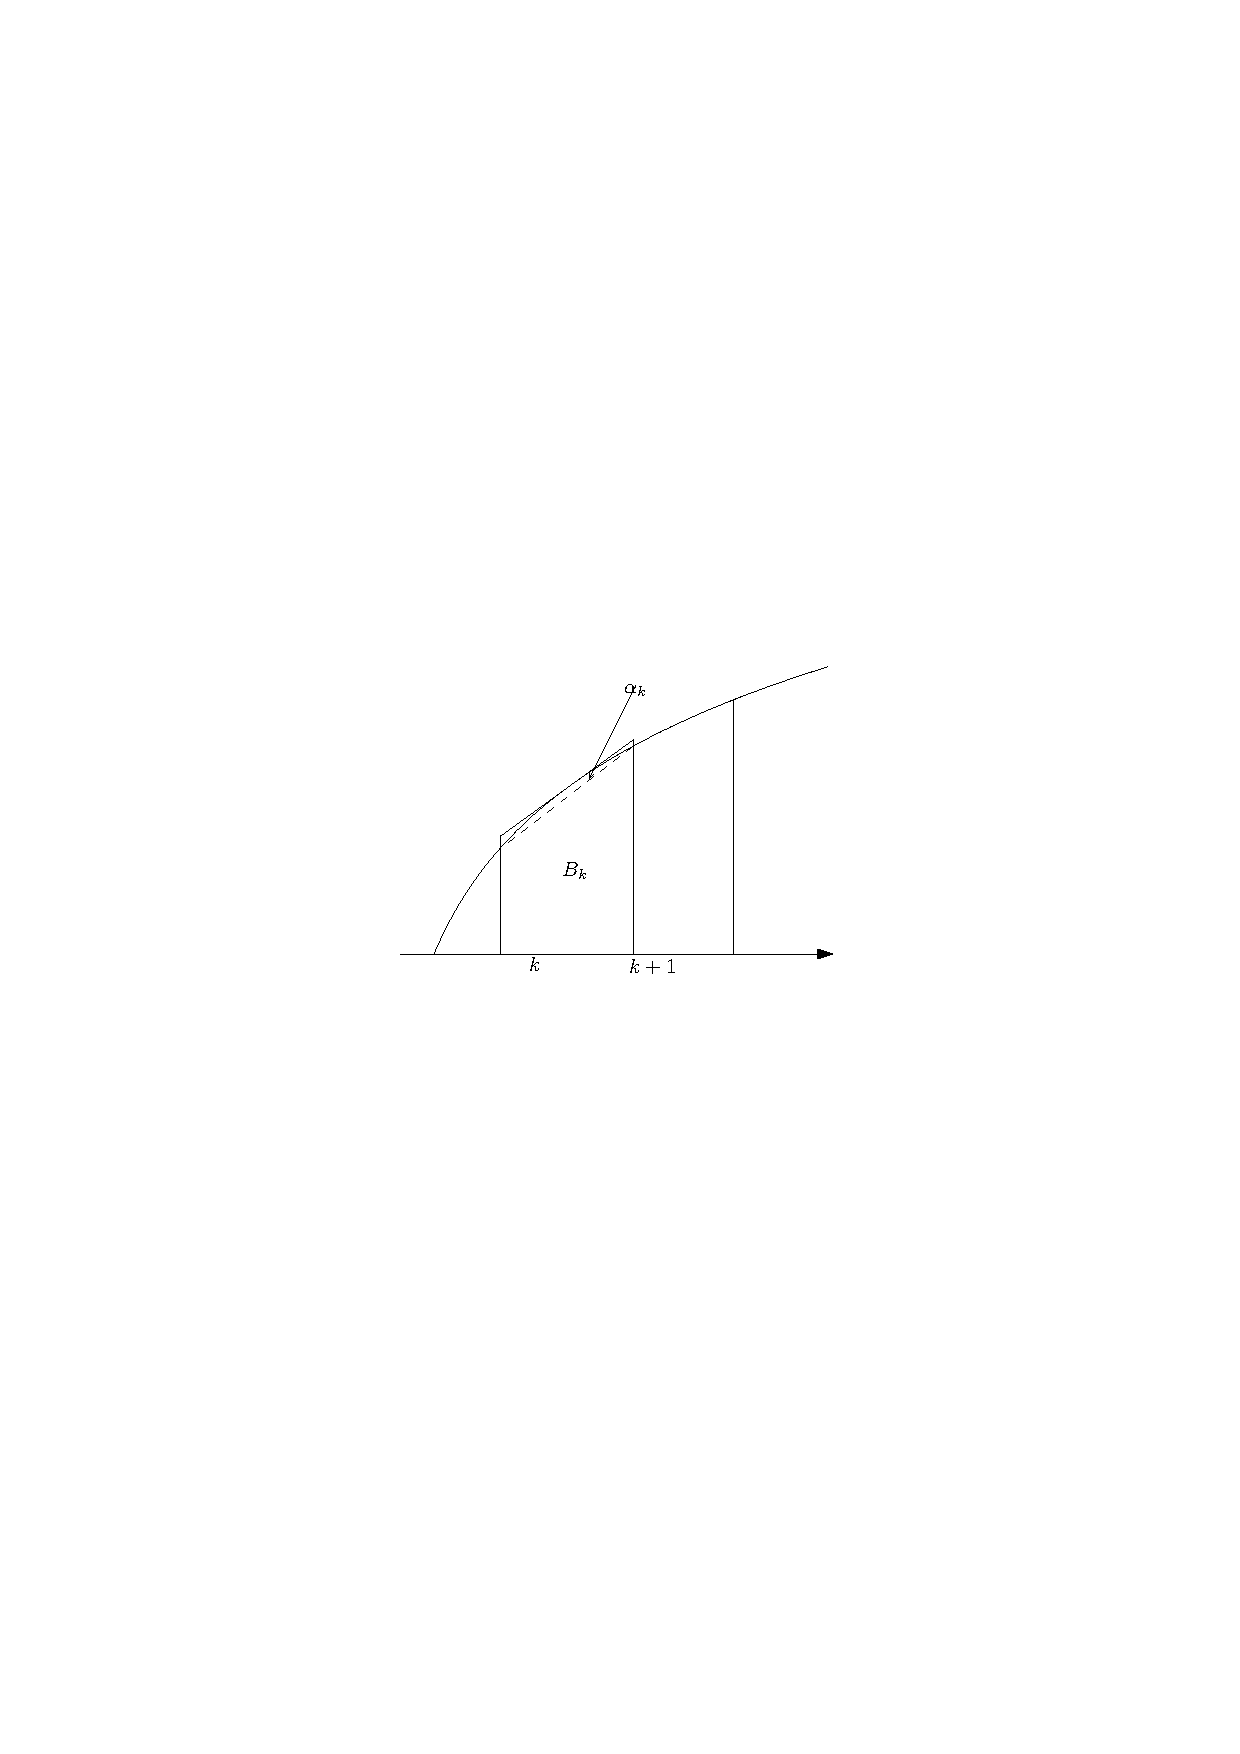
\includegraphics[width=0.5\linewidth]{stirllog}
    \caption{К формуле Стирлинга}
    \label{fig:stirform}
  \end{figure}

  \begin{align*}
    \intertext{Нормальная площадь:}
    A_n &= \int_{1}^{n} \ln x\, dx = \left. ( x \ln x \vphantom{\int} - x)\right|_1^n = n \ln n - n + 1 \\
    \intertext{Приближение:} 
    B_n &= \sum_{k=1}^{n} \left( \frac{\ln(k+1) + \ln(k)}{2} \right) = \ln n! - \frac{1}{2} \ln n \\
    \intertext{Кусочки можно оценить сверху маленькими трапециями, касание там в центре промежутка:} 
    \alpha_k &= \int_k^{k+1} \ln x \, dx - \frac{1}{2} (\ln k + \ln (k+1)) 
    < \ln \left( k + \frac{1}{2} \right) - \frac{1}{2} \big(\ln k + \ln(k+1)\big) \\
    &= \frac{1}{2}\left( \ln\left(1 + \frac{1}{2k}\right) - \ln\left(1+\frac{1}{2k+1}\right) \right)
  \end{align*}
  А тогда $\sum \alpha_k$~--- ряд Лейбница, и 
  \[
    \sum \alpha_k \in \left[0;\frac{1}{2}\ln\lfrac{3}{2}\right], 
    \quad \frac{1}{2} \ln \left( 1 + \frac{1}{2n} \right)  > r_n > 0.
  \]
  Остаток положительный, так как первый член остатка ряда положителен.
  Дальше много преобразований...
  \begin{align*}
    n \ln n - n + 1  - \ln n! + \frac{1}{2} \ln n &= \alpha - r_n \Leftrightarrow \\
    \ln n! &= \left( n+\frac{1}{2} \right) \ln n - n + (1 - \alpha) - r_n 
  \end{align*}
  Теперь разберёмся с остатком
  \[
    e^{r_n} < e^{\frac{1}{2} \ln \left( 1+ \frac{1}{2n} \right)} = \sqrt{1 + \frac{1}{2n}} < 1 + \frac{1}{4n}
  \]
  Таким образом,
  \[
    e^{r_n} = \left( 1 + \frac{\theta}{4n} \right), \;\; \theta\in (0;1)
  \]
  если теперь ещё заменить $c = e^{1-\alpha}$, то получится формула~\ref{thrm:stirform}.
\end{ittproof}
\begin{rem}
  Если приближать не трапециями, а параболами, то можно получить и третью. 
\end{rem}
\begin{thrm}
  Константа $c$ в формуле Стирлинга равна $\sqrt{2\pi}$
\end{thrm}
\begin{ittproof}
  Формулой Валлиса(\ref{thrm:wallisf}) пробьётся.
\end{ittproof}

%<+welcome-to-endofsyn+>
\end{document}


\chapter{Функциональные ряды}
\documentclass[12pt]{../../notes}
\usepackage{silence}
\WarningFilter{latex}{Reference}
\graphicspath{{../../img/}}
\begin{document}

\paragraph{Равномерная сходимость}
\begin{defn}\label{defn:pointconv}
  Пусть $X \subset \R$, $f, f_n\colon X\to \R$. Тогда говорят, что $f_n \to f$ \emph{поточечно}, если
  \[
    \Big( 
      \forall\, x\in X \; \forall\, \varepsilon > 0 \; \exists\, N(\varepsilon,x) :
      \forall\, n > N \; |f_n(x) - f(x)| < \varepsilon  
    \Big) \Leftrightarrow
    f_n \to f
  \]
\end{defn}

\begin{defn}\label{defn:uniconv}
  Пусть $X \subset \R$, $f, f_n\colon X\to \R$. Тогда говорят, что $f_n$ сходится к $f$ \emph{равномерно}, если
  \[
    \Big( 
      \forall\, \varepsilon > 0 \; \exists\, N(\varepsilon) :
      \forall\, x \in X \; \forall\, n > N \; |f_n(x) - f(x)| < \varepsilon  
    \Big) \Leftrightarrow
    f_n \overset{X}{\rightrightarrows} f
  \]
\end{defn}
\begin{exmp*}
  $X = [0;1]$, $f_n(x) = x^n$. При этом
  \[
    \lim_{n\to \infty} f_n(x) = f(x) 
    = \begin{cases}
        0, x < 1 \\
        1, x = 1
      \end{cases}
  \]
  Достаточно взять $\varepsilon$ равным $\lfrac{1}{2}$ чтобы понять что с равномерной сходимостью проблемы.
\end{exmp*}

\begin{defn}\label{defn:tchdev}
  Пусть $f,g\colon X \to \R$. Тогда 
  \[
    \rho(f,g):= \sup_{x\in X} |f(x) - g(x)|
  \]
  называется чебышёвским уклонением.
\end{defn}

\begin{stat}\label{stat:uniconvsign}
  \[
    f_n \overset{X}{\rightrightarrows} f \Leftrightarrow \rho(f_n, f) \to 0
  \]
\end{stat}

\paragraph{Теорема о непрерывности предельной функции}
\begin{thrm}\label{thrm:uniconvcont}
  Пусть $\forall\, n \; f_n \in C(I)$, $f_n \overset{I}{\rightrightarrows} f$. Тогда и $f \in C(I)$
\end{thrm}
\begin{ittproof}
  Скомбинировав определения непрерывности и равномерной сходимости, получим что такое:
  \[
    |f(x) - f(x_0)| = |f(x) - f_n(x) + f_n(x) - f_n(x_0) + f_n(x_0) - f(x_0)| < 3\varepsilon
  \]
\end{ittproof}

\paragraph{Предельный переход под знаком производной и интеграла}
\begin{thrm}\label{thrm:uniconvint}
  Пусть $\forall\, n \; f_n \in C(I)$,$I=[a;b]$, $f_n \overset{I}{\rightrightarrows} f$. 
  Тогда
  \[
    \int_{a}^{b} f_n \to \int_{a}^{b} f
  \]
\end{thrm}
\begin{ittproof}
 \[
   \left| \int_a^b f_n - \int_a^b f \right| = \left| \int_a^b (f_n - f) \right| \leqslant 
  \int_a^b |f_n - f| < \varepsilon (b - a) = \varepsilon_1
 \]
\end{ittproof}


\begin{thrm}\label{thrm:uniconvder}
  Пусть $\forall\, n \; f_n \in C^1(I)$, $f_n \rightarrow f$, $f_n' \overset{I}{\rightrightarrows} \varphi $.
  Тогда $\varphi \in C^0(I)$, $\varphi = f$
\end{thrm}
\begin{ittproof}
  Через теорему Барроу сводится к теореме~\ref{thrm:uniconvint}
\end{ittproof}

\begin{rem*}
  Поточечной сходимости не хватит, например $f_n(x) = \frac{1}{n} \arctg(nx)$ в нуле.
\end{rem*}

Таким образом, три предыдущие теоремы можно (подразумевая соответствующие условия) коротко записать так:
\begin{table}[h!]
  \begin{tabular}{ll}
    \ref{thrm:uniconvcont} 
    & $\displaystyle \lim_{t\to x} \lim_{n\to \infty} f_n(t) = \lim_{n\to \infty} \lim_{t\to x} f_n(t) $ \\
    \ref{thrm:uniconvint} 
    & $\displaystyle \int_a^b \lim_{n\to \infty} f_n(x) \, dx = \lim_{n\to \infty} \int_a^b f_n(x) \, dx$ \\
    \ref{thrm:uniconvder} 
    & $\displaystyle \frac{\mathrm{d}}{\mathrm{d}x} \lim_{n\to \infty} f_n(x) 
    = \lim_{n\to \infty} \frac{\mathrm{d}}{\mathrm{d}x} f_n(x) $
  \end{tabular}
\end{table}

\paragraph{Равномерная сходимость функциональных рядов}

\begin{defn}\label{defn:convfseries}
  Функциональный ряд называется сходящимся при таком-то $x$, если частичные суммы сходятся поточечно.
\end{defn}

\begin{defn}\label{defn:uniconvfseries}
  Функциональный ряд $\sum u_n(x)$ называется равномерно сходящимся на $X$, 
  если $S_n(x) \overset{X}{\rightrightarrows} S$
\end{defn}

\subparagraph{Несколько свойств:}
\begin{enumerate}
  \item $\sum u_n(x)$ равномерно сходится на $X$ $\Rightarrow u_n(x)\overset{X}{\rightrightarrows} 0 $
  \item $\sum_{n=1}^\infty u_n(x)$ и $\sum_{n=m}^\infty u_n(x)$ имеют одинаковый характер равномерной сходимости на
    $X$
  \item $\sum u_n(x)$ равномерно сходится на $X$ $\Leftrightarrow$
    \[
      \forall\, \varepsilon \;\: \exists\, N \colon \forall\, n > N \;\: \forall\, p > 0 \;\: \forall\, x\in X \;\:
      \left| \sum_{k=n+1}^{n+p} u_k (x) \right| < \varepsilon
    \]
    Докажем последний пункт веселья ради

    \begin{itlproof}
      Сначала перепишем условие равномерной сходимости:
      \[
        \begin{split}
          S_n(x) = \sum_{k=1}^n u_k(x) \overset{X}{\rightrightarrows} S(x) \Leftrightarrow \\
          \forall\, \varepsilon \;\: \exists\, N \colon \forall\, x \; \forall n > N \;\: |S_n(x)-S(x)| < \varepsilon
        \end{split}
      \]
      \begin{description}
        \item[\circlearound{$\Rightarrow$}] Заметим, что
          \[
            \left| \sum_{k=n+1}^{n+p} u_k(x) \right| = | S_{n+p}(x) - S_n(x) |
          \]
          Тогда из равномерной сходимости:
          \[
            | S_{n+p}(x) - S_n(x) | = |S_{n+p}(x) - S(x)| + |S_n(x) - S(x)| < 2\varepsilon
          \]
        \item[\circlearound{$\Leftarrow$}] Тут есть поточечная сходимость, 
          по такому же критерию для рядов~\ref{stat:bkseriesconv}.
          Таким образом, $S_{n+p}(x)\xrightarrow[p\to \infty]{} S(x)$.
          А значит из условия признака
          \[
            \forall\, \varepsilon \;\: \exists\, N \colon \forall\, n > N \;\: 
            \forall\, p > 0 \;\: \forall\, x\in X \;\:
            \left| S(x) - S_n(x) \right| \leqslant \varepsilon < 2\varepsilon
          \]
      \end{description}
    \end{itlproof}
\end{enumerate}

\begin{thrm}[Признак равномерной сходимости Вейерштрасса]\label{thrm:uniconvseriesweir}
  Пусть $\sum u_n(x)$, $x\in X$, и, также, $\exists\, (c_n) \colon$
  \begin{enumerate}
    \item $\forall\, x\in X \; \forall n\in \N \;\: |u_n(x)| \leqslant c_n$
    \item $\sum c_n$ сходится
  \end{enumerate}
  Тогда $\sum u_n(x) $ равномерно сходится на $X$
\end{thrm}
\begin{ittproof}
  \[
    \left| \sum_{k=n+1}^{n+p} u_k(x) \right| \leqslant\sum_{k=n+1}^{n+p}| u_k(x) | \leqslant \sum_{k=n+1}^{n+p} c_k 
    < \varepsilon
  \]
\end{ittproof}

\begin{thrm}[Признак Дирихле]\label{thrm:uniconvseriesdir}
  Пусть есть функциональный ряд $\sum u_n(x)\cdot\nolinebreak v_n(x)$, $x\in X$. Пусть к тому же
  \begin{enumerate}
    \item $u_n(x) \overset{X}{\rightrightarrows} 0 $, $u_n \searrow$
    \item $\exists\, M \colon \forall\, x\in X \; |v_1(x) + \dotsb + v_n(x)| \leqslant M$.
  \end{enumerate}
  Тогда $\sum u_n(x) $ равномерно сходится на $X$
\end{thrm}

\begin{thrm}[Признак Абеля]\label{thrm:uniconvseriesabel}
  Пусть есть функциональный ряд $\sum u_n(x)\cdot\nolinebreak v_n(x)$, $x\in X$. Пусть к тому же
  \begin{enumerate}
    \item $u_n(x)$ монотонна по $n$ при фиксированном $x$ и равномерно ограничена на $X$ 
      ( $\exists\, M\colon \forall\, x \in X \; \forall\, k \in \N \;\: |u_n(x)| \leqslant M$ ).
    \item $\sum v_k(x)$ равномерно сходится на $X$.
  \end{enumerate}
  Тогда $\sum u_n(x) $ равномерно сходится на $X$
\end{thrm}

\paragraph{Свойства суммы функционального ряда}
\begin{thrm}\label{thrm:uniconvseriescont}
  Пусть есть функциональный ряд $\sum u_n(x)$, $x\in X$. Пусть к тому же
  \begin{enumerate}
    \item $u_n(x)$ непрерывна на $X$
    \item $\sum u_n(x)$ равномерно сходится на $X$
  \end{enumerate}
  Тогда $S(x) = \sum u_n(x)$ непрерывна на $X$
\end{thrm}

\begin{ittproof}
  Про сумму конечного числа функций это правда. А дальше~---  следствие~\ref{thrm:uniconvcont}.
\end{ittproof}

\begin{thrm}\label{thrm:uniconvseriesint}
  Пусть есть функциональный ряд $\sum u_n(x)$, $x\in X$. Пусть к тому же
  \begin{enumerate}
    \item $u_n(x)$ непрерывна на $X$
    \item $\sum u_n(x)$ равномерно сходится на $X$
  \end{enumerate}
  Тогда 
  \[
    \int_X \sum_\N u_n(x) dx = \sum_\N \int_X u_n(x) dx 
  \]
  То есть ряд можно почленно интегрировать.
\end{thrm}

\begin{ittproof}
  Про сумму конечного числа функций это правда. А дальше~---  следствие~\ref{thrm:uniconvint}.
\end{ittproof}

\begin{thrm}\label{thrm:uniconvseriesderiv}
  Пусть есть функциональный ряд $\sum u_n(x)$, $x\in X$, $u_n\in~C^1(X)$. Пусть к тому же
  \begin{enumerate}
    \item $\sum u_n(x)$ сходится на $X$ поточечно
    \item $\sum u_n'(x)$ равномерно сходится на $X$
  \end{enumerate}
  Тогда $S(x) = \sum u_n(x)$ дифференцируема на $X$ и
  \[
    \frac{\mathrm{d}}{\mathrm{d}x}\left( \sum_\N u_n(x) \right) = \sum_\N \frac{\mathrm{d}}{\mathrm{d}x} u_n(x)
  \]
  То есть ряд при соблюдении определённых условий можно почленно дифференцировать. 
\end{thrm}

\begin{ittproof}
  Про сумму конечного числа функций это правда. А дальше~---  следствие~\ref{thrm:uniconvder}.
\end{ittproof}

\paragraph{Пределы и ряды в \texorpdfstring{$\C$}{}}
\begin{defn}\label{defn:complim}
  Пусть $(z_k)\in~\C$. Тогда $z_k = x_k + i y_k$, где $x_k,y_k~\in~\R$, а $|z_k|=\sqrt{x_k^2+y_k^2}$.
  Предел определим так:
  \[
    z = \lim_{k\to \infty} z_k \Leftrightarrow \forall\,\varepsilon > 0 \; \exists\, N \colon 
    \forall\, k > N \; |z_k - z| < \varepsilon
  \]
\end{defn}
\begin{thrm}\label{thrm:compcoordlim}
  Пусть $z=(x,y) = (r,\varphi)$, $z_k = (x_k, y_k) = (r_k, \varphi_k)$. Тогда
  \begin{align*}
    z_k \to z \Leftrightarrow \begin{cases} x_k\to x \\ y_k\to y \end{cases} \\
    z_k \to z \Leftarrow \begin{cases} r_k\to r \\ \varphi_k\to \varphi \end{cases} \\
  \end{align*}
\end{thrm}
\begin{ittproof}
  С одной стороны 
  \[
    |z_k - z| \leqslant |x_k - x| + |y_k - y| 
  \]
  С другой стороны
  \[
    \begin{cases}
      &|z_k - z| \geqslant |x_k - x| \\
      &|z_k - z| \geqslant |y_k - y|
    \end{cases}
  \]
  В полярном представлении это следует из непрерывности, пользоваться ей уже в принципе можно, предел
  определён ведь.
\end{ittproof}
\begin{rem*}
  В полярном представлении нету равносильности, так как, например, можно накручивать спираль на $(0;0)$
  и поломать при этом $\varphi$
\end{rem*}
\begin{defn}\label{defn:compseries}
  Пусть $(z_k)\in~\C$, 
  \[
      S_n = \sum_{k=1}^{n} z_k = \sum_{k=1}^{n} x_k + i \sum_{k=1}^{n} y_k
  \]
  Тогда
  \[
      S = \sum_{k=1}^{\infty} z_k := \sum_{k=1}^{\infty} x_k + i \sum_{k=1}^{\infty} y_k  
  \]
\end{defn}
\begin{defn}\label{defn:complderiv}
  Пусть $u: \C \to \C$. Тогда
  \[
    u'(z) := \lim_{h\to 0} \frac{u(z+h) - u(z)}{h}
  \]
\end{defn}
Теперь можно относительно безболезненно поверить во все ранее доказанные свойства и для $\C$.
Дальше ряды будут в основном из $\C$, но всё то же самое будет верно и для $\R$

\paragraph{Степенные ряды. Теорема об области сходимости}
\begin{defn}\label{defn:powerseries}
  Такой функциональный ряд: $\sum c_k z^k$, где $c_k,z\in\C$ называется степенным рядом.
  Множество $\{z\in\C \mid \sum c_k z^k \conv\}$~--- область сходимости. 
\end{defn}

\begin{thrm}[Формула Коши-Адамара]\label{thrm:circleconv}
  Пусть есть степенной ряд $\sum c_k z^k$ и ещё несколько хитрых чисел:
  \begin{align*}
    &\ell := \uplim_{k\to \infty}{\root k \of {|c_k|}}, \; \ell \in [0;+\infty] &\\
    &R := \begin{cases}
      +\infty, & \ell = 0 \\
      \lfrac{1}{\ell}, & 0 < \ell < +\infty \\
      0, & \ell = +\infty
    \end{cases}&
  \end{align*}
  Тогда:
  \begin{enumerate}
    \item $|z| < R \Rightarrow \sum |c_k x^k| \conv$
    \item $|z| > R \Rightarrow \sum c_k x^k \noconv$
    \item $|z| = R $~--- ничего не понятно
  \end{enumerate}
  Таким образом, степенной ряд сходится абсолютно в круге. А вот что происходит на границе 
  Ойкумены, этот признак не знает.
\end{thrm}
\begin{ittproof}
  Усиленный признак сходимости Коши(\ref{thrm:enhcauchyconv}) поможет делу.
\end{ittproof}

\begin{rem*}
  Можно переехать из нуля в произвольную точку, тогда там просто всюду будет $|z-a|$ вместо $|z|$.
\end{rem*}

\begin{thrm}[О равномерной сходимости степенного ряда]\label{thrm:uniconvpowerseries}
  Пусть есть степенной ряд $\sum c_k (z-a)^k$, $R\in(0;+\infty)$
  \begin{enumerate}
    \item Пусть $r\colon 0 < r < R$. Тогда ряд $\sum c_k (z-a)^k$ равномерно сходится в $B_r$.
    \item Пусть $z_0$ лежит на границе круга и $\sum c_k (z-a)^k$ сходится в точке $z_0$.
      Тогда ряд равномерно сходится на радиусе
      \[
        \{ z \mid z = a + \theta(z_0 - a), \theta \in [0;1] \}
      \]
  \end{enumerate}
\end{thrm}
\begin{ittproof}
  \begin{enumerate}
    \item Признак Вейерштрасса~\ref{thrm:uniconvseriesweir} поможет тут.
    \item Немного перепишем:
      \[
        u_k(z) =  c_k(z-a)^k = \underbrace{\theta^n} \underbrace{c_k (z_0 - a)^k} 
      \]
      Первая часть монотонна по $n$ и равномерно ограничена единицей. А сумма второй равномерно
      \footnote{ну она вообще от $x$ не зависит} сходится по предположению. Таким образом, 
      $\sum u_k(z)$ сходится равномерно на $[a;z_0]$
  \end{enumerate}
\end{ittproof}

\begin{rem*}
  Вообще, последний пункт верен для любого $z_0\in \C$, главное, чтобы в нём была сходимость
  \marginpar{\small см.~\cite[стр.~448]{zorich2}}
\end{rem*}

\paragraph{Свойства суммы степенного ряда}

\begin{thrm}\label{thrm:powerseriescont}
  Пусть $S(z) = \sum c_k (z-a)^k$~--- степенной ряд, $R\in~(0;+\infty)$
  Тогда
  \begin{enumerate}
    \item $S$ непрерывна в $\mathcal{D}_r = \{z \mid |z-a|\leqslant r\}\; \forall\, r\in (0;R)$
    \item ряд сходится в $z_0$ $\Rightarrow$ 
      \[
        S(z_0) = \lim_{\theta \nearrow 1-0} S(a + \theta(z_0-a))
      \]
  \end{enumerate}
\end{thrm}

\begin{thrm}\label{thrm:powerseriesint}
  Пусть $S(z) = \sum c_k (z-a)^k$~--- степенной ряд, $R\in(0;+\infty)$, $I=[z_1; z_2]\in$ области сходимости.
  Тогда
  \begin{enumerate}
    \item $|z_1 - a| < R \wedge |z_2 - a| < R$ $\Rightarrow$ 
      \[
        \int_I S(z)\,dz = \sum_{k=0}^\infty \int_I c_k (z - a)^k\,dz
      \]
    \item $z_2 \colon |z_2 - a| = R$, $J = [a;z_2]$ 
      \[
        \int_J S(z)\,dz = \sum_{k=0}^\infty \int_J c_k (z - a)^k\,dz
      \]
  \end{enumerate}
\end{thrm}
{\small
Скорее всего, вот это место никто кроме меня внимательно читать не будет.
Так что
\begin{verse}
Четырнадцать студентов \\
Пришли матан сдавать. \\
Не все вели конспекты \\
И их осталось пять. \\
\end{verse}
Однако, продолжим.
}

\begin{thrm}\label{thrm:powerseriesder}
  Пусть $S(z) = \sum c_k (z-a)^k$~--- степенной ряд, $R\in(0;+\infty)$
  Тогда $\forall\, z\colon |z-a| < R \;\: S'(z)$ сходится в круге с таким же радиусом и
  \[
    S'(z) = \sum_{k=1}^{\infty} c_k \cdot k (z-a)^{k-1} 
  \]
\end{thrm}
\begin{ittproof}
  Нетрудно показать из \ref{thrm:circleconv}, что радиус круга сходимости для ряда из производных такой же.
  А дальше комбинируя \ref{thrm:uniconvseriesderiv} и \ref{thrm:uniconvpowerseries} получаем, что надо.
\end{ittproof}

\parrange{2}{Ряды Тейлора}

\begin{defn}[Ряд Тейлора]\label{defn:taylorseries}
  Пусть $f\in C^\infty(I)$. Тогда
  \[
    T(x) := \sum_{k=0}^{\infty} \frac{f^{(k)}(a)}{k!}\,(x-a)^k
  \]
\end{defn}

\begin{lem}\label{lem:taylresid}
  В какой-то фиксированной точке $x$ функция совпадает с разложением 
  $\Leftrightarrow$ $R_n(x) \xrightarrow[n\to\infty]{} 0$.
\end{lem}

\begin{lem}\label{lem:taylpowlim}
  Пусть на всем интервале $I\subset\R$ 
  \[
    \exists\, M\colon \forall\,x \in I \; \forall\,n \;\: |f^{(n)}(x)| \leqslant M^n 
  \]
  Тогда функция совпадает со своим разложением в ряд на $I$.
\end{lem}
\begin{itlproof}
  Можно оценить остаток, представив его в форме Лагранжа, и оно к нулю сойдётся, так как
  факториал убывает быстрее показательной функции.
\end{itlproof}

\begin{thrm}[Единственность степенного разложения]\label{thrm:powerseriesuniq}
  Пусть $f(x) = \sum c_n x^n$. Тогда $\{c_i\}$~--- коэффициенты Тейлора.
\end{thrm}
\begin{ittproof}
  Достаточно посчитать производные в нуле, они совпадут с $c_i$-ыми.
\end{ittproof}

\begin{defn}\label{defn:funanalit}
  Говорят, что функция аналитична в $z_0\in\C$, если в $V(z_0)$.
  \[
    f(z) = \sum_{n=0}^{\infty} c_n (z-z_0)^n
  \]
\end{defn}

Теперь можно раскладывать в ряд, всё нужные инструменты для этого есть.

\begin{table}[h]
  \caption{Разложение всяких функций в ряд}
  \label{tab:taylorseries}
  \vspace{1ex}
  \centering
  \begin{tabular}{lll}
    $f(x)$      & $S(x)$                                                  & Область сходимости \\[0.3em]
    $\sin x$    & $\dsum_{k=0}^{\infty} \frac{(-1)^k}{(2k+1)!}\,x^{2k+1}$ & $\R$ \\[0.3em]
    $\cos x$    & $\dsum_{k=0}^{\infty} \frac{(-1)^k}{(2k)!}\,x^{2k}$     & $\R$ \\[0.3em]
    $e^x$       & $\dsum_{k=0}^{\infty} \frac{1}{k!}\,x^{k}$              & $\R$ \\[0.3em]
    $\ln x$     & $\dsum_{k=1}^{\infty} \frac{(-1)^{k-1}}{k!}\,x^{k}$     & $(-1;1]$ \\[0.3em]
    $(1+x)^\mu$ & $\dsum_{k=0}^{\infty} \binom{\mu}{k}\,x^{k}$            & $(-1;1)$
  \end{tabular}
\end{table}


\begin{lem}\label{lem:sinseries}
  Функции $\sin x$ и $\cos x$ раскладываются как указано в таблице~$\ref{tab:taylorseries}$. 
\end{lem}
\begin{itlproof}
  $f^{(n)}(x)$~--- это либо синус либо косинус с каким-то знаком. 
  Во всяком случае $\forall\,x \in \R\;$ $|f^{(n)}(x)|\leqslant 1$.
  А тогда по лемме~\ref{lem:taylpowlim} оно всё совпадает со своим разложением на $\R$. 
\end{itlproof}

\begin{lem}\label{lem:expseries}
  Функции $\exp x$ раскладываются как указано в таблице $\ref{tab:taylorseries}$. 
\end{lem}
\begin{itlproof}
  На любом конечном интервале $[-\infty;a]$ есть сходимость. А для любой точки из $\R$ можно
  найти содержащий её (даже вместе с некой окрестностью) конечный интервал. Таким образом, $\exp x$ аналитична 
  на $\R$.
\end{itlproof}


\begin{itlproof}[Разложение логарифма]
  Считать много производных тут неприятно. Зато можно почленно интегрировать и дифференцировать.
 
  В круге с радиусом 1 вот такой степенной ряд сходится равномерно:
  \[
    f'(x) = 1 - x + x^2 - x^3 + \dotsb = \frac{1}{1+x}\text{ (геометрическая прогрессия) }
  \]
  Теперь можно его проинтегрировать (на отрезке $[0;x]$, $x\in (-1,1)$, например).
  \[
    f(x) = x - \frac{x^2}{2} + \frac{x^3}{3} - \frac{x^4}{4} + \dotsb = \ln (1+x)
  \]
  Заметим, что такой ряд сходится в $x_0 = 1$. А значит, на отрезке $[0;1]$ есть равномерная сходимость.
  А тогда по непрерывности $f(1)=\ln 2$. 
\end{itlproof}

\begin{itlproof}[Разложение степенной функции]
  Тут проще сразу взять ряд из таблицы~\ref{tab:taylorseries}, доказать, что он сходится равномерно 
  в круге радиусом 1 и , затем, убедиться, что он удовлетворяет соотношению
  \[
    (1+x) S'(x) = \mu S(x)
  \]
  откуда уже следует, что это степенной ряд. 
  Значение в нуле~--- 1 , так что произвольная константа окажется равной 0.
\end{itlproof}

\paragraph{Экспонента и тригонометрия в \texorpdfstring{$\C$}{}}
\begin{defn}\label{defn:expsincompl}
  Определим $\forall\,z\in \C$
  \begin{align*}
    \sin z & := \dsum_{k=0}^{\infty} \frac{(-1)^k}{(2k+1)!}\,z^{2k+1}  \\
    \cos z & := \dsum_{k=0}^{\infty} \frac{(-1)^k}{(2k)!}\,z^{2k}   \\
    \exp z & := \dsum_{k=0}^{\infty} \frac{1}{k!}\,z^{k}
  \end{align*}
\end{defn}

Из такого определения вытекают следующие свойства:
\begin{enumerate}
  \item $\forall\, z_1, z_2\in \C \;\: \exp(z_1+z_2) = \exp(z_1) + \exp(z_2)$
  \item $\forall\, x\in \R \;\: \exp(x) = e^x$
  \item $\forall\, x,y \in \R \;\: \exp(x+iy) = e^x(\cos y + i \sin y)$. В частности 
    \fbox{$e^{i\pi} + 1 = 0$} (Формула Эйлера)
  \item $\sin$ и $\cos$ можно выразить так:
    \begin{align*}
      \sin z &= \frac{1}{2i}\big(\exp(iz) - \exp(-iz)\big) \\[0.3em]
      \sin z &= \frac{1}{2}\big(\exp(iz) + \exp(-iz)\big) \\
    \end{align*}
  \item 
    \(\displaystyle 
      \begin{aligned}
        \sin(z_1 + z_2) &= \sin z_1 \cos z_2 + \cos z_1 \sin z_2\\
        \sin(z_1 + z_2) &= \cos z_1 \cos z_2 - \sin z_1 \sin z_2\\
      \end{aligned}
    \)
  \item $\exp z$~--- периодична с $T_0 = 2\pi i$
\end{enumerate}

Ещё интересно заметить, что экспонента переводит прямоугольные координаты в полярные.
А полярные координаты немного неоднозначны. Это к тому, что комплексный логарифм неоднозначен.

\paragraph{Логарифм комплексного аргумента}

\begin{defn}[Комплексный логарифм]\label{defn:compllog}
  $\forall\, w \neq 0 \;\: e^z = w$ имеет решение, правда неоднозначное.
  \[
    z_k = \ln |w| + i (\arg w + 2\pi k), \; k\in \Z
  \]
  Таким образом:
  \begin{align*}
    \ln w &= \ln |w| + i \arg w \text{~--- главное значение логарифма } \\
    \Ln w &= \{\ln |w| + i (\arg w + 2\pi k) \mid k\in \Z \}
  \end{align*}
\end{defn}

\paragraph{Понятие непрерывной ветви логарифма и корня}

\textbf{Осторожно! Дальше лажа!}

Посмотрим на функцию $f(z) = \ln z = \ln |z| + i \arg z$. Она была бы всем хороша
и непрерывна, если бы при обходе нуля угол внезапно не перескакивал из-за того, что $\arg z \in[-\pi;\pi]$.
А непрерывности хочется.

\begin{defn}\label{defn:logcontbranch}
  Пусть $G \subset \C$ , $f \colon G \to \C$, $f\in C(G)$. Тогда $f$~--- непрерывная ветвь логарифма, если 
  $\forall\, z\in G \;\: \exp f(z) = z$.
\end{defn}

\begin{thrm}
  \begin{enumerate}
    \item В $\C \setminus \R_+$ бесконечно много ветвей логарифма.
    \item В $\C \setminus {0}$ их нет вовсе.
  \end{enumerate}
\end{thrm}
Нужно было как-то запретить обход нуля, в первом случае это у нас получилось.

\begin{defn}[Комплексная степень]\label{defn:complpower}
  \[
    z_1^{z_2} := \{ z \mid z = e^{z_2(\ln z_1 + 2\pi i k )} \}
  \]
\end{defn}

\begin{defn}\label{defn:rootcontbrnch}
  Пусть $G \subset \C$ , $f \colon G \to \C$, $f\in C(G)$. Тогда $f$~--- непрерывная ветвь корня $n$ степени,
  если $\forall\, z\in G \;\: f(z)^n = z$.
\end{defn}

Тут надо бы ещё про римановы поверхности сказать, но не вышло у меня $\ddot\frown$.
Я лучше картинок вставлю.
\begin{figure}
  \begin{minipage}{0.49\linewidth}
    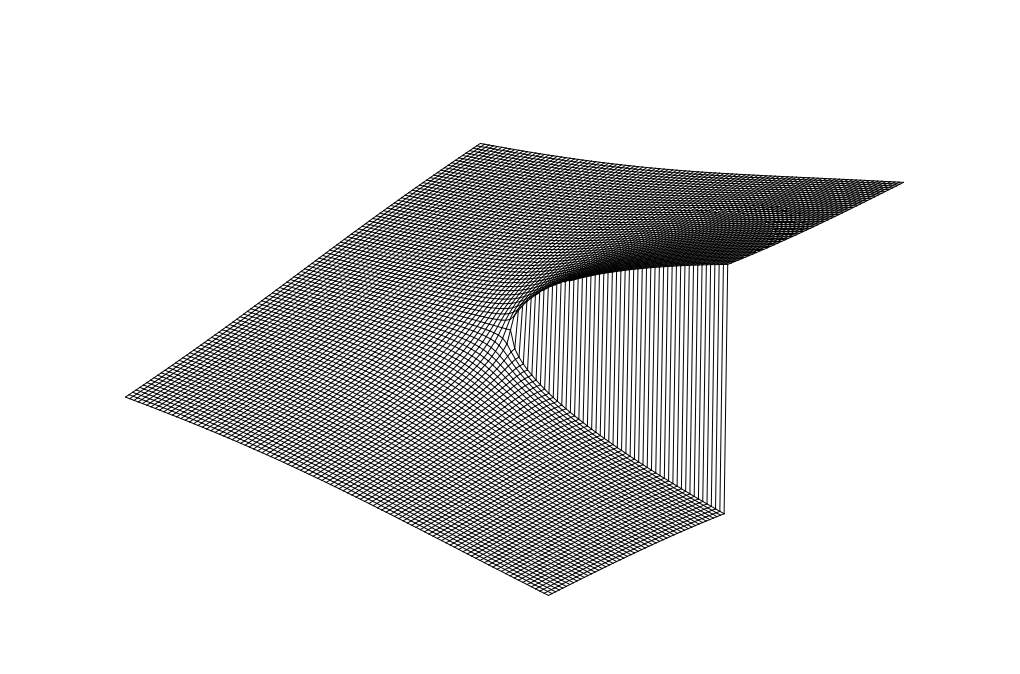
\includegraphics[width=1\linewidth]{sqrprobl}
  \end{minipage} \hfill
  \begin{minipage}{0.49\linewidth}
    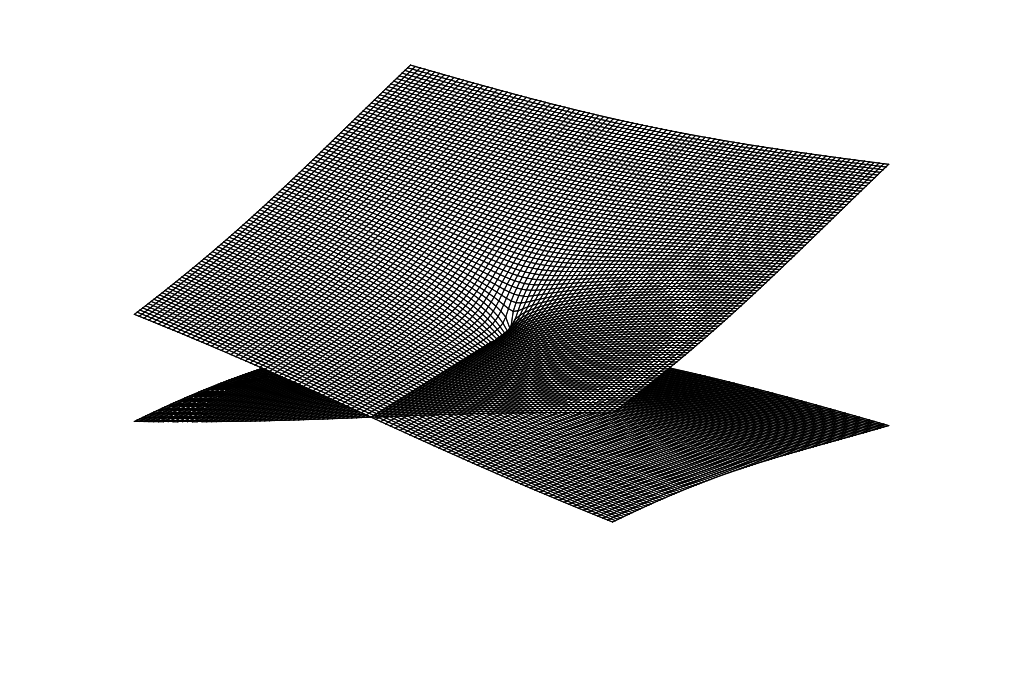
\includegraphics[width=1\linewidth]{sqrootrim}
  \end{minipage}
  \caption{Разрыв мнимой части у корня и риманова поверхность для него}
  \label{fig:sqrtrimsurf}
\end{figure}

\begin{figure}[h]
  \centering
  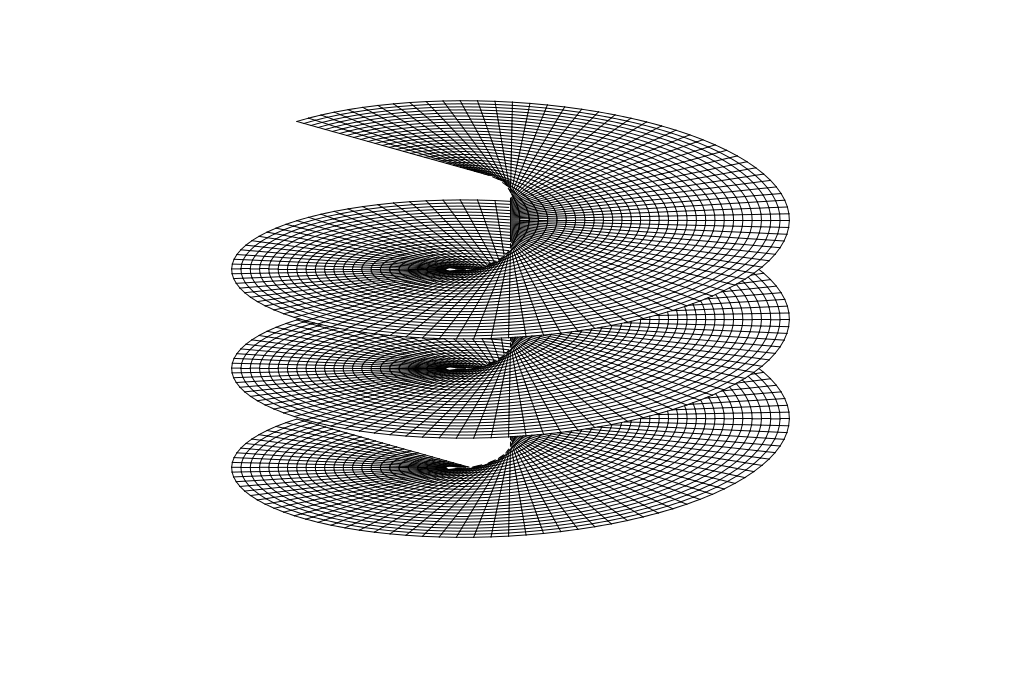
\includegraphics[width=0.8\linewidth]{logrimsurf}
  \caption{Риманова поверхность для логарифма}
  \label{fig:logrimsurf}
\end{figure}




























% <+endofspell+> 
\end{document}


\chapter{Дифференциальное исчисление в \texorpdfstring{$\R^n$}{R\^{}n}}
\documentclass[12pt]{../../notes}
\usepackage{silence}
\WarningFilter{latex}{Reference}
\graphicspath{{../../img/}}
\begin{document}

\paragraph{Основные структуры в \texorpdfstring{$\R^n$}{R\^{}n}}

\begin{defn}\label{defn:Rn}
  $\R^n = \{ (x^1, \dotsc, x^n) \mid x^1, \dotsc, x^n \in \R \}$. Сделаем теперь из $\R^n$ векторное пространство
  над $\R$
  введя соответствующие операции. В дальнейшем будем работать с $\R^n$ уже как с векторным пространством.
\end{defn}

\begin{defn}\label{defn:scalprodRn}
  Пусть $x, y\in \R^n$. Тогда скалярное произведение $\langle x,y\rangle$ определяется как
  операция со следующими свойствами:
  \begin{enumerate}
    \item $\langle \alpha x + \beta y , z \rangle = \alpha \langle x,y\rangle + \beta \langle y,z\rangle$
    \item $\langle x , y \rangle = \langle y, x\rangle$
    \item $\forall\, x \in \R^n, x > 0 \;\; \langle x , x \rangle > 0$
  \end{enumerate}
  В частности, в ортонормированном базисе 
  \[
    \langle x, y \rangle = \sum_{i=1}^{n} x^i y^i
  \]
\end{defn}
\begin{defn}\label{defn:normRn}
  Пусть $x\in \R^n$. Тогда определим норму в $\R^n$ так:
  \[
    \| x \| = \sqrt{\langle x,x \rangle} = \sqrt{\sum_{i=1}^{n} x_i^2}
  \]
  Свойства нормы:
  \begin{enumerate}
    \item $\forall\, x\in \R^n \;\: \| x \| \geqslant 0$, $\|x\| = 0 \Leftrightarrow x = 0$
    \item $\forall\, \alpha\in\R, x\in \R^n \;\; \|\alpha x\| = |\alpha| \cdot \|x\|$
    \item $\forall\, x, y \in \R^n \;\: \|x + y\| \leqslant \|x\| + \|y\|$
  \end{enumerate}
  Последнее (котрое неренство треугольника) верно по неравенству Минковского,
  которое следствие неравенства Гёльдера. 
\end{defn}

\begin{defn}[Метрика в $\R^n$]\label{defn:rhoRn}
  $\forall\, x, y \in \R^n \;\: \rho(x,y) := \| x - y \|$, $\rho$~--- эвклидово расстояние.
  Про него верны следующие свойства:
  \begin{enumerate}
    \item $\forall\, x, y \in \R^n \;\: \rho(x,y) = \rho(y,x)$
    \item $\forall\, x, y \in \R^n \;\:\rho(x,y) \geqslant 0$, $\rho(x,y) = 0 \Leftrightarrow x = y $
    \item $\forall\, x, y, z \in \R^n \;\:\rho(x,y) \leqslant \rho(x,z) + \rho(z,y)$
  \end{enumerate}
\end{defn}

\begin{defn}\label{defn:metrspace}
  $(\R^n, \rho)$~--- метрическое пространство.
\end{defn}

\begin{rem*}
  Наверное было бы лучше определить и норму и метрику через их свойста, так более общо. 
  А потом доказать, что и евклидова норма и евклидова метрика являются нормой и метрикой, соответственно.
  Но вроде не нужно, к тому же мне лень править этот кусок.
\end{rem*}

\begin{defn}[Шар в $\R^n$]\label{defn:ballRn}
  Пусть $a\in \R^n$, $r > 0$.
  \[
    B_r(a) := \{ x\in \R^n \mid \rho(x,a) < r \}
  \]
\end{defn}

\begin{defn}\label{defn:openRn}
  Множество $G \subset \R^n$~--- открытое, если 
  \[
    \forall\, a \in G \; \exists\, B_r(a) \colon B_r(a) \subset G
  \]
  Если $G_1, \dotsc, G_n$~--- открытые множества, то и $\bigcap\limits_{1\leqslant i \leqslant n} G_i$ ,
  $\bigcup\limits_{1\leqslant i \leqslant n} G_i$~--- открытые.
\end{defn}

\begin{exmp*}
  Шар в $\R^n$~--- открытое множество.
\end{exmp*}

\begin{defn}\label{defn:topology}
  Топология на множестве $X$~--- такое семейство множеств $T \subset 2^X$, что 
  \begin{enumerate}
    \item $\varnothing \in T$
    \item $X \in T$
    \item $A_1, \dotsc, A_n \in T \Rightarrow \bigcap\limits_{1\leqslant i \leqslant n} A_i$
    \item $A_1, \dotsc, A_n \in T \Rightarrow \bigcup\limits_{1\leqslant i \leqslant n} A_i$
  \end{enumerate}
  Элементы семейства называются открытыми множествами.
\end{defn}

\begin{exmp}
  $T = \{ X, \varnothing \}$~--- тривиальная (антидискретная) топология на $X$.
\end{exmp}

\begin{exmp}
  Открытые множества, как мы их определили в~\ref{defn:openRn} задают стандартную топологию на $\R^n$
\end{exmp}

\begin{defn}[Окрестность в $\R^n$]\label{defn:neightbRn}
  Пусть $x\in \R^n$. Тогда $U(x)$~--- произвольное открытое множество, содержащее $x$. 
\end{defn}
\begin{exmp*}
  В качестве окрестности подойдёт $B_\varepsilon$, например.
\end{exmp*}
\begin{rem*}
  Проколотая окрестность определяется всё так же: $\overset{\circ}{U}(x) = U \setminus \{x\}$.
\end{rem*}

\begin{defn}[Предел в $\R^n$]\label{defn:limtop}
  Пусть $x_k\in \R^n$, $a\in \R^n$. Тогда 
  \[
    \lim_{k\to \infty} x_k = a \Leftrightarrow \forall\, U(a) \;\: \exists\, N\colon
    \forall\, k > N \;\: x_k \in U(a)
  \]
  Теперь для функций. 
  Пусть $f\in X \subset \R^n \to \R^m$, $x_0$~--- точка сгущения $X$, $A\in \R^m$. Тогда 
  \[
    \lim_{x\to x_0} f(x) = A \Leftrightarrow \forall\, \overset{\circ}{U(A)} \;\:
    \exists\, \overset{\circ}{V(x_0)} \colon x\in \overset{\circ}{V} \Rightarrow f(x) \in \overset{\circ}{U}
  \]
\end{defn}

\begin{stat}[Свойства предела в $\R^n$]\label{stat:limcoordRn}
  $x_k \to a \Leftrightarrow \rho(x,a) \to 0 \Leftrightarrow \| x_k - a \| \to 0$.
  И тогда 
  \[
    \lim_{k\to \infty} x_k = a \Leftrightarrow \forall\, i \;\: x_k^i \to a^i
  \]
  То есть сходимость в $\R^n$ покоординатная. 
\end{stat}
\begin{itlproof}
  Тут на самом деле 2 утверждения:
  \begin{enumerate}
    \item $x_k \to a \Leftrightarrow \rho(x, a) \to 0$.
      \begin{description}
        \item[\circlearound{$\Leftarrow$}] Из определения открытого множества в любой окрестности $x_0$ 
          есть шар $B_\varepsilon(x_0)$. А если принадлежит шару, то и окрестности.
        \item[\circlearound{$\Rightarrow$}] $B_\varepsilon(a)$~--- тоже окрестность. 
      \end{description}
    \item $ x_k \to a \Leftrightarrow \forall\, i \;\: x_k^i \to a^i$
      \begin{description}
        \item[\circlearound{$\Leftarrow$}] Ясно из того, как задана норма в $\R^n$~(\ref{defn:normRn}).
        \item[\circlearound{$\Rightarrow$}] Многомерный параллелепипед~--- тоже окрестность. 
      \end{description}
  \end{enumerate}
\end{itlproof}


\paragraph{Секвенциальная компактность}

\begin{defn}[Предельная точка]\label{defn:limpoint}
  Пусть $X \subset \R^n$, $a\in \R^n$ Тогда $a$~--- предельная точка $X$, если 
  $\exists\, (x_n)\in X \colon x_n \to a$
\end{defn}

\begin{rem*}
  При таком определении предельная точка $\neq$ точка сгущения
\end{rem*}

\begin{exmp*}
  $X = \{a\}$~--- есть последовательность $(x_n) \equiv a$, сходящаяся к $a$, но
  $\overset{\circ}{V}(a) = \varnothing$
\end{exmp*}

\begin{defn}\label{defn:closedRn}
  Пусть $X\subset \R^n$. Тогда $X$~--- замкнуто, если содержит все свои предельные точки
\end{defn}

\begin{defn}[Замыкание]\label{defn:closureRn}
  Пусть $X \subset \R^n$. Тогда $\overline{X} = \clos(X)$~--- множество всех предельных точек $X$.
\end{defn}

\begin{exmp*}
  $\clos \Q = \R$
\end{exmp*}

Свойства замыкания:
\begin{enumerate}
  \item $\varnothing$ замкнуто
  \item $\R^n$ замкнуто
  \item объединение и пересечение замкнутых множеств замкнуто
\end{enumerate}

\begin{thrm}\label{thrm:closopenRn}
  Пусть $G \subset \R^n$, $F = \R^n \setminus G$. Тогда $G$ открыто $\Leftrightarrow$ $F$ замкнуто.
\end{thrm}

\begin{defn}\label{defn:seqcompRn}
  Пусть $X\subset \R^n$. Тогда $X$~--- компактное, если 
  \[
    \forall\, (x_m) \in X \; \exists\, (x_{m_k}) \colon x_{m_k} \to c , c \in X
  \]
  То есть, в нём выполняется принцип Больцано-Вейерштрасса.
\end{defn}

\begin{defn}\label{defn:limitedsetRn}
  Множество $X\subset \R^n$~--- ограниченно, если 
  \[
    \sup_{x_1, x_2 \in X} \rho (x_1, x_2) \in \R
  \]
\end{defn}

\begin{thrm}\label{thrm:compclosopenRn}
  Пусть $X\subset \R^n$. Тогда $X$~--- компактно $\Leftrightarrow$ $X$ замкнуто и ограничено.
\end{thrm}
\begin{ittproof}
  \begin{description}
    \item[\circlearound{$\Rightarrow$}] Проблемы с пределом последовательности
    \item[\circlearound{$\Leftarrow$}] Можно мнооого раз применять одномерную теорему Больцано-Коши
      для каждого измерения и оно получится.
  \end{description}
\end{ittproof}
\begin{rem*}
  Не работает в бесконечномерных
\end{rem*}

\paragraph{\texorpdfstring{$\R^n$}{R\^{}n} как полное метрическое пространство}

\begin{defn}\label{defn:cauchyseq}
  Последовательность $(x_n)$ называется фундаментальной (последовательностью Коши),
  если 
  \[
    \forall\, \varepsilon > 0 \;\: \exists\, N\colon \forall\,m,n>N \;\: \rho(x_n - x_m) < \varepsilon 
  \]
\end{defn}

\begin{defn}\label{defn:comtmetspc}
  Метрическое пространство $(X,\rho)$~--- полное, если всякая фундаментальная последовательность
  в нём  сходится
\end{defn}

\begin{exmp*}
  $\R \setminus 0$~--- не полное метрическое пространство, $x_n = \lfrac{1}{n}$ тому пример.
\end{exmp*}

\begin{stat}\label{stat:comtRn}
  $\R^n$~--- полное метрическое пространство.
\end{stat}
\begin{itlproof}
  $\sphericalangle$ произвольный $\varepsilon > 0$. Тогда 
  \[
    \rho(x_n - x_m) < \varepsilon 
    \Rightarrow \forall\, i \;\: \rho(x_m^i e_i - x_n^i e_i) < \varepsilon
    \Rightarrow \forall\, i \;\: |x_m^i - x_n^i| < \varepsilon
  \]
  Таким образом $(x_n^i)\in \R$~--- фундаментальная. 
  А в $\R$ по теореме из первого семестра фундаментальные последовательности сходятся.
  Тогда $\forall\, x_n^i \to a^i$. Значит и $x_n \to a$ по теореме~\ref{stat:limcoordRn}
\end{itlproof}

\paragraph{Непрерывные отображения}

\begin{defn}\label{defn:contRn}
  Пусть $f\colon X \subset \R^n \to \R^m$. Тогда $f$ непрерывна в $x_0\in X$, если
  \[
    \forall\, U\big(f(x_0)\big) \; \exists\, V(x_0) \colon x \in V \Rightarrow f(x) \in U
  \]
  Можно например в качестве окрестности брать $B_\varepsilon$.
\end{defn}

%\begin{stat}\label{stat:contcoordRn}
  %Аналогично пределу, непрерывность в $\R^n$ имеет покоординатный характер.
%\end{stat}
\begin{defn}\label{defn:openinsubsetRn}
  Множество $A\subset X \subset \R^n$ называется открытым в $G$, если 
  \[
    \forall\, a\in A \;\: \exists B_r(a) \colon B_r(a) \cap X \subset A
  \]
\end{defn}

\begin{thrm}\label{thrm:contopen}
  Пусть $f\colon X \subset \R^n \to \R^m$~--- непрерывна, тогда и только тогда, когда
  \[
    \forall\, G\subset \R^m \colon G\text{~--- открытое } \;\: f^{-1}(G)\text{~--- открытое в }X
  \]
\end{thrm}
\begin{ittproof}
  \begin{description}
    \item[\circlearound{$\Rightarrow$}] Пусть $f(x) = y\in G$  Тогда из открытости $G$ 
      \[
        \exists\,B_\varepsilon(y) \colon B_\varepsilon(y) \subset G
      \]
      Но из непрерывности
      \[
        \forall\, B_\varepsilon(y) \;\: \exists\, B_\delta(x) \colon \forall\, x'\in B_\delta \cap X 
        \;\: y'=f(x') \in B_\varepsilon 
      \]
      А раз $f(x')\in B_\varepsilon \subset G$, то $x'\in f^{-1}(G)$. То есть 
      \[
        \forall\, x \in f^{-1}(G) \;\: \exists\,B_\delta(x) \colon \forall\, x'\in B_\delta \cap X 
        \;\: x'\in f^{-1}(G)
      \]
      А это как раз открытость $f^{-1}(G)$ в $X$.
    \item[\circlearound{$\Leftarrow$}] Пусть $y = f(x)$. Рассмотрим тогда $B_\varepsilon(y)$.
      Оно открыто, и, по условию, $f^{-1}(B_\varepsilon)$~--- открыто в $X$. Тогда 
      \[
        \forall\, x'\in f^{-1}(B_\varepsilon) \;\: \exists B_\delta(x') \colon
        B_\delta(x') \cap X \subset f^{-1}(B_\varepsilon) 
      \]
      Но в таком случае
      \[
        \forall\, x'' \in B_\delta(x') \cap X \;\: f(x'') \in B_\varepsilon
      \]
  \end{description}
\end{ittproof}

\begin{imp}\label{stat:contsuperpos}
  $f, g$~--- непрерывны, $f\circ g$ определена $\Rightarrow$ $f\circ g$ непрерывна.
\end{imp} 

\begin{thrm}[Вейерштрасса]\label{thrm:weierRn}
  Пусть $f\colon X \subset \R^n \to \R^m$, $X$~---компакт. 
  Тогда $f\in C(x) \Rightarrow  f(X)$~--- компактно.
\end{thrm}
\begin{ittproof}
  Можно рассмотреть какую-нибудь последовательность в $f(X)$ и  вытащить сходящуюся подпоследовательность
  из её прообраза. А тогда по непрерывности образ подпоследовательности сходится к чему-то в $f(X)$.
  А значит оно компактно.
\end{ittproof}

\begin{imp}
  При $m=1$ $f$ ограничена и достигает своего минимума/максимума
\end{imp}

\begin{itlproof}
  Ограниченность очевидна, а супремум и инфимум~--- предельные точки.
\end{itlproof}

\begin{defn}\label{defn:unicontRn}
  Пусть $f\colon X \subset \R^n \to \R^m$. Тогда $f$ равномерно непрерывна на $X$, если
  \[
    \forall\, \varepsilon \; \exists\, \delta(\varepsilon) \colon \forall\,x,x_0\in X 
    \;\:\| x - x_0 \| \Rightarrow \| f(x) - f(x_0) \|
  \]
\end{defn}

\begin{thrm}[Кантора]\label{thrm:cantRn}
  $f\in C(X), X$~--- компакт $ \Leftrightarrow$ $f$ равномерно непрерывна на $X$.
\end{thrm}
\begin{ittproof}
  Так же, как и в одномерье~--- от противного; следствие принципа выбора Больцано-Вейерштрасса.
\end{ittproof}

\begin{thrm}[Больцано-Коши]\label{thrm:bolzcauchyRn}
  Пусть $f : X\subset \R^n\to \R$, $f\in C(X)$ и $\forall\,a,b \in X $ $\exists\,\Gamma \in X \colon$
  $\Gamma$~--- непрерывная кривая, содержащая $a, b$, и $f(a)\cdot f(b) < 0$. Тогда
  $\exists\, c \in X \colon f(c) = 0$.
\end{thrm}
\begin{ittproof}
  Следствие непрерывности композиции и одномерной теоремы Больцано-Коши.
\end{ittproof}

\begin{thrm}\label{thrm:coordfcontRn}
  \[
    f \in C(x_0) \Leftrightarrow \forall\, i \;\: f^i \in C(x_0)
  \]
\end{thrm}
\begin{ittproof}
  Вообще-то, свойство предела. См.~\ref{stat:limcoordRn}.
\end{ittproof}

\paragraph{Соотношение между непрерывностью по каждому аргументу и непрерывностью по совокупности переменных}

Это не то же самое, что непрерывность по каждой координатной функции, надо это понимать. Я вот только
сейчас (2016-06-09 01:43) понял это совсем хорошо.

\begin{defn}\label{defn:contargRn}
  Отображение $f_j: X\subset\R^n \to R$ непрерывно по $i$-ой координате в точке $x_0$, если 
  \[
    \begin{split}
      \forall\, \varepsilon > 0 \;\: \exists\, \delta > 0 \colon &| x^i - x^i_0 | < \delta \Rightarrow \\ 
      &\Rightarrow | f_j(x_0^1, \dotsc, x^i, \dotsc, x^n_0) - f_j(x_0^1, \dotsc, x^i_0, \dotsc, x^n_0)  | <\varepsilon
    \end{split}
  \]
\end{defn}

\begin{lem}\label{lem:contfandcontargRn}
  Отображение $f_j: X\subset\R^n \to R$ непрерывно точке $x_0$, $\Rightarrow$ $f_j$ непрерывно по каждому аргументу.
  Обратное неверно, см.~пример~\ref{exmp:partialinsuff}
\end{lem}

%\begin{thrm}\label{thrm:contargproperRn}
  %Если $f: \R^n \to \R$ непрерывна по каждому аргументу в $U(x_0)$, то $f$ непрерывна в $x_0$.
%\end{thrm}

%\begin{ittproof}
  %Можно поочерёдно переходить к пределам по координатам в окрестности $x_0$ и вроде выйдет. А если
  %она изолированная, то там по определению всё непрерывно.
%\end{ittproof}

\parrange{2}{Линейное отображение и его норма}

Вспомним определение из алгебры:
\begin{defn}\label{defn:linfun}
  Пусть $\varphi:V \to U$, $V,U$~--- линейные пространства и
  \begin{enumerate}
    \item $\varphi(x+y) = \varphi(x) + \varphi(y)$
    \item $\varphi(\alpha x) = \alpha \varphi(x)$
  \end{enumerate}
  Тогда $\varphi$~--- линейное отображение.
\end{defn}

\begin{rem}
  В дальнейшем $\varphi : \R^n \to \R^m$ всюду будет линейным отображением,
  так что выберем в $\R^n$ стандартный базис и обозначим матрицу $\varphi$ в нём за $A$.
\end{rem}

\begin{defn}[Норма линейного отображения]\label{defn:normlinfun}
  \[
    \| A \| := \sup_{\substack{x \in \R^n \\ x\neq 0}} \frac{\|Ax\|}{\|x\|}
  \]
\end{defn}
\begin{lem}\label{lem:normnormlinfun}
  \[
    \sup_{x \neq 0}  \frac{\|Ax\|}{\|x\|}  = \sup_{\|x'\|=1} \|Ax'\|
  \]
\end{lem}

\begin{thrm}[Об оценке нормы линейного отображения]\label{thrm:apprnormlinfun}
  Пусть $A = (a_{ij})$, тогда
  \[
    \| A \| \leqslant \sqrt{\sum_{i,j}a_{ij}^2}
  \]
\end{thrm}
\begin{ittproof}
  Неравенство Коши-Буняковского в чистом виде.
\end{ittproof}

\subparagraph{ Свойства нормы линейного отображения:}
\begin{enumerate}
  \item $\|A\| > 0; \; \|A\|=0 \Leftrightarrow A\equiv 0$
  \item $\forall\,\alpha \in \R\;\: \|\alpha A\| = |\alpha| \|A\|$
  \item $\varphi,\psi:\R^n \to \R^m$ $\|A+B\| \leqslant \|A\| + \|B\|$
  \item $\displaystyle
    \begin{aligned}
      &\varphi : \R^n \to \R^m \\
      &\psi: \R^m \to \R^p
    \end{aligned}$, $\psi \circ \varphi : \R^m \to \R^p$ $\|BA\| \leqslant \|B\|\,\|A\|$.
\end{enumerate}
\begin{itlproof}
  Основные инструменты доказательства~--- свойства нормы и неравенство $\| Ax \| \leqslant \|A\|\,\|x\|$, очевидно следующее
  из определения~\ref{defn:normlinfun}
\end{itlproof}

\begin{stat}\label{stat:lincont}
  Линейное отображение непрерывно
\end{stat}
\begin{itlproof}
  Пусть $A$~--- матрица линейного отображения $\R^n \to \R^m$, $x_0$~--- точка сгущения.
  Тогда при $x \to x_0$ :
  \[
    0 \leqslant \| Ax - Ax_0 \| = \| A(x-x_0) \| \leqslant \|A\| \, \|x - x_0\| \to 0
  \]
  Так можно, ведь норма отображения ограничена из~\ref{thrm:apprnormlinfun}.
\end{itlproof}

\paragraph{Дифференцируемость отображения}
\begin{defn}\label{defn:diffRn}
  Пусть $f:\R^n \to \R^m$. Тогда $f\in C^1(x)$ если 
  \begin{align}
    & \exists\, \varphi_A:\R^n \to \R^m \colon \Delta f(x,h) = \mathrm{A} h + \alpha(h)\label{eq:difffun} \\
    & \alpha(h) = o(h) \Leftrightarrow \frac{\alpha(h)}{\|h\|} \xrightarrow[h\to 0]{} 0
  \end{align}
\end{defn}
\begin{rem*}
  Вообще, смещение $h$ тут может быть любым. Например в частных производных меняется всего одна координата.
\end{rem*}

\begin{stat}\label{stat:diffcontRn}
  $f \in C^1(x) \Rightarrow f \in C^0(x)$
\end{stat}

\begin{stat}[Покоординатный характер сходимости]\label{stat:diffcorrd}
  Пусть $f: X \subset \R^n \to \R^m$ , $x\in X$, $y = f(x) = (y_1,\dotsc,y_n)$, $y^i = f_i(x)$.
  
  Тогда 
  \[
    f\in C^1(x) \Leftrightarrow \forall\, i \;\: f^i \in C^1 (x^i)
  \] и 
  \[
    \Delta f^i = \sum_{j=1}^{n} a_{ij}h^j + o(h^j)
  \]
\end{stat}

\begin{itlproof}
  Распишем равенство \eqref{eq:difffun} через координатные функции, которые вещественнозначные :
  \[
    \begin{cases}
      \Delta f^1 = f^1(x + h) - f^1(x) = A^1 h + \alpha^1(x,h)&\\
      \hdotsfor{1} &\\
      \Delta f^m = f^m(x + h) - f^m(x) = A^m h + \alpha^m(x,h)&
    \end{cases}
  \]
  где $A = (A^1, \dotsc, A^m)$~--- все очевидно линейные функции. Также очевидно, что 
  \[
    \frac{\alpha}{\|h\|} \to 0 \Leftrightarrow \forall\, i \frac{\alpha}{\|h\|} \to 0 
  \]
  Ну а тогда координатные функции дифференцируемы.
  Если ещё вспомнить, чему равны $A^i$, получится оставшаяся часть утверждения.
\end{itlproof}

\begin{defn}[Частная производная]\label{defn:partial}
  $f:X \subset \R^n \to R$, $x$~--- внутренняя точка $X$.
  \[
    \frac{\partial f}{\partial x^i}(x) 
    := \lim_{t \to 0} \frac{f(x^1, \dotsc, x^i + t, \dotsc, x^n) - f(x^1, \dotsc, x^n)}{t}
  \]
\end{defn}

\begin{rem*}
  \[
    \frac{\partial f}{\partial x^i}(x) \equiv \partial_i f \equiv \mathcal{D}_i f \equiv f_{x^i}'
  \]
\end{rem*}

\begin{thrm}[Единственность линейной части приращения]\label{thrm:diffcoefpart}
  $f : X \subset \R^n \to \R \in $ дифференцируема в $x$ $\Rightarrow$ 
  \[
    \exists\, \{a_i\} \colon \Delta f = \sum_{i=1}^{n} a_i h^i + o(h^i) , \; a_i = \partial_i f(x)
  \]
  То есть $a_i$ определяются однозначно.
\end{thrm}
\begin{ittproof}
  Получится, если рассмотреть 
  \[
    h = (0, \dotsc, t, \dotsc, 0)
  \]
  и из определения частной производной~\ref{defn:partial} $a_i$ как раз и получаются каким надо$b$
\end{ittproof}

\begin{rem*}
  Обратное утверждение неверно, существования всех частных производных не хватит для дифференцируемости.
\end{rem*}
\begin{exmp}\label{exmp:partialinsuff}
  \[
    f = \begin{cases}
      1, &xy \neq 0 \\
      0, &xy = 0
    \end{cases}
  \]
\end{exmp}

\begin{imp}
  Пусть теперь $f:\R^n \to R^m$. Тогда $f^i : \R^n \to \R$. Таким образом $a_{ij} = \partial_j f^i(x)$.
\end{imp}

\paragraph{Дифференциал}

\begin{defn}\label{defn:derivativeRn}
  Производную $f'(x)$ можно теперь определить так:
  \[
    f'(x) := A = (a_{ij}) = 
    \begin{pmatrix}
      \partial_1 f^1(x) & \cdots & \partial_n f^1(x) \\
      \vdots            & \ddots & \vdots \\
      \partial_1 f_m(x) & \cdots & \partial_n f_m(x) \\
    \end{pmatrix}
  \]
  где $A$~--- матрица Якоби
\end{defn}

\begin{defn}\label{defn:differentialRn}
  Дифференциал $\mathrm{d}(f,h)$ определим так:
  \[
    \mathrm{d}f(x) := \mathrm{d}(f,h):= A h = 
    \begin{pmatrix}
      \partial_1 f^1(x) & \cdots & \partial_n f^1(x) \\
      \vdots         & \ddots & \vdots \\
      \partial_1 f_m(x) & \cdots & \partial_n f_m(x) \\
    \end{pmatrix}\cdot
    \begin{pmatrix}
      h^1 \\
      \vdots \\
      h^n \\
    \end{pmatrix}, \; h = \Delta x = dx
  \]
\end{defn}

Ещё видимо тут должно быть вот это утверждение:~\ref{thrm:diffcoefpart}
\paragraph{Достаточное условие дифференцируемости}

\begin{thrm}\label{thrm:nessdiffRn}
  Пусть $f:G \subset \R^n \to \R$, $a \in G$. Пусть также в некоторой окрестности $U(a)$ $\exists\, \partial_i f(x)$
  и они непрерывны в $a$. Тогда $f$ дифференцируема в $a$.
\end{thrm}
\begin{ittproof}
  Не успею написать нормально, но расписать приращение , а потом применить теорему Лагранжа и \emph{аккуратно} перейти к пределам\ldots
\end{ittproof}

\begin{defn}\label{defn:smoothRn}
  Пусть $f:G\subset \R^n \to \R$. Пусть также в $G$ существуют и непрерывны все $\partial_i f$.
  Тогда отображение $f$ называется \emph{гладким} \\ $\big(f\in C^1(G;\R^n)\big)$.
\end{defn}

\paragraph{Свойства дифференцируемых отображений}
\begin{enumerate}
  \item $f \in C^1 \Rightarrow f \in C^0$
  \item $(\alpha f + \beta g)'(x) = \alpha f'(x) + \beta g'(x)$
  \item $f, g: \R \to \R^n$ $\langle f,g\rangle' = \langle f',g\rangle + \langle f,g'\rangle $
  \item $f, g: \R^n \to \R$  $(fg)' = f'g + fg'$
  \item $f, g: \R \to \R^3$  $(f \times g)' = f' \times g + f \times g'$
\end{enumerate}

\begin{itlproof}
  Дифференцируемость всего следует из того, что производная~--- матрица.
  Все произведения тоже линейны. Получится короче, просто писать некогда.
\end{itlproof}

\paragraph{Правило цепочки}

\begin{thrm}\label{stat:diffsuperpRn}
  Пусть $f : X \subset \R^n \to \R^m$, $g : Y \subset \R^m \to \R^p$, $f(X) \subset Y$.
  Пусть также $f \in C^1(x), g \in C^1(\,f(x)\,)$. 

  Тогда $(g \circ f) \in C(x)$ и $(g\circ f)' = g'\circ f \cdot f'$. (Это таки произведение матриц)
\end{thrm}

\begin{ittproof}
  Посмотрим на приращение:
  \[
    \begin{split}
      \Delta (g \circ f) &= (g \circ f)(x+h) - (g \circ f)(x) = g(\underbrace{f(x+h)}_{y+k}) - g(\underbrace{f(x)}_{y}) \\ 
          &= \mathrm{B} k + \beta = \mathrm{B}(\mathrm{A} h + \alpha ) + \beta 
          = \mathrm{B}\mathrm{A} h + \underbrace{\mathrm{B} \alpha + \beta}_\gamma
    \end{split}
  \]
  Здесь $B = g'(y)$, $A = f'(x)$.
  Осталось доказать, что $\gamma = o(\|h\|)$. 

  Сначала заметим, что $\mathrm{B}$~--- ограничена $\Rightarrow \mathrm{B} \alpha = \mathrm{B} o(\|h\|) = o(\|h\|)$.
  Теперь надо пострадать. Потому что $k = 0$ бывает.

  Сначала рассмотрим случай $k \neq 0$.
  \[
    \| k \| = \| A h + \alpha \| \leqslant \|A\| \cdot \|h\| + \|\alpha\| = O(\|h\|) 
  \]
  Тогда
  \[
    \beta = o(\|k\|) = o(O(\|h\|)) = o(\|h\|)
  \]
  В случае же $k = 0$ ничего существенно не изменится, можно просто доопределить $\beta(0) = 0$ 
  (ну и правда, $\beta = (\Delta g - B\cdot k)(0) = 0$).
\end{ittproof}

\begin{imp}[Правило цепочки]\label{stat:chainrule}
  Пусть $y^i = f^i(x^1, \dotsc, x^n)$, $z^i = f^i(y^1, \dotsc, y^m)$
  \[
    \frac{\partial z^i}{\partial x^j} = \sum_{k=1}^{m} \left( \frac{\partial z^i}{\partial y^k}(y) 
        \cdot \frac{\partial y^k}{\partial x^j}(x) \right)
  \]
\end{imp}

\paragraph{Касательные к кривым на поверхности}

\begin{stat}\label{stat:tanplane}
  Пусть $S = f(x,y)$. Это какая-то поверхность а $p = (x^0, y^0, z^0)$, $z^0 = f(x^0, y^0)$~--- точка на
  ней. Тогда уравнение касательной плоскости(непонятно что это, но вроде из геометрии видно) можно записать как-то так
  \[
    z - z^0 = \frac{\partial f}{\partial x}(x^0)\cdot(x-x^0) + \frac{\partial f}{\partial y}(y^0)\cdot(y-y^0) 
  \]
\end{stat}


\begin{stat}\label{stat:curvetanRn}
  Пусть $\Gamma$~--- кривая в $S\subset\R^3$, а $S = f(x,y)$. Пусть на этой кривой есть точка 
  $p = (x^0, y^0, z^0)$, $z^0 = f(x^0, y^0)$, а $T$~--- касательная плоскость к $S$ в $p$.
  Тогда если $L$~---  касательная к $\Gamma$, то $L \subset T$
\end{stat}


\paragraph{Признак постоянства функции в области}
\begin{defn}\label{defn:spaceRn}
  Область~--- открытое связное множество
\end{defn}

\begin{thrm}\label{thrm:signconstRn}
  Пусть $f:G\subset\R^n \to \R$, $f\in C^1(G)$. Пусть также в $G$ $\forall\, \partial_i f \equiv 0$.
  Тогда $f \equiv const$
\end{thrm}
\begin{ittproof}
  В области можно любые 2 точки соединить путём $\gamma : [0;1] \to \R^n$. Теперь, если рассмотреть $F = f \circ \gamma$, то
  ситуация сведётся к одномерному случаю.
\end{ittproof}

\paragraph{Производная по вектору}
\begin{defn}\label{defn:vecderivRn}
  Пусть $f:G\subset\R^n \to \R$, $G$~--- открытое, $a\in G$, $v \in \R^n$. Тогда
  \[
    \mathcal{D}_v f(a) := \lim_{t\to 0} \frac{f(a+tv)-f(a)}{t}\text{~--- производная по вектору $v$ }
  \]
  (если существует, конечно)
\end{defn}

\begin{defn}\label{defn:gradRn}
  $\grad f = \nabla f := (\partial_1 f, \dotsc, \partial_n f)$~--- градиент $f$. Вообще его в целом 
  лучше определять как-то более инвариантней, но пока и так сойдёт.
\end{defn}

\begin{thrm}[Связь с градиентом]\label{thrm:gradvecderRn}
  Пусть $f\in C(a)$. 
  \[
    \forall\, v\in \R^n \;\: \exists\, \mathcal{D}_v f(a) 
    \wedge \bigg( \mathcal{D}_v f(a) = \langle \nabla f(a) , v \rangle \bigg)
  \]
\end{thrm}
\begin{ittproof}
  Рассмотрим $F(t) = f(x(t)) = f(a + t v)$. Тогда по правилу цепочки
  \[
    \mathcal{D}_v = F'(0) = \sum_{k=1}^n \frac{\partial f}{\partial x^k}(x(0) = a)\cdot \frac{\partial x^k}{\partial t} 
    = \langle \nabla f, v\rangle
  \]
\end{ittproof}

\begin{rem}
  Если рассмотреть всевозможные $v:\|v\|=1$, то получится, что функция быстрей всего возрастает в 
  направлении градиента со ``скоростью'' $\|\nabla f(a)\|$ соответственно
\end{rem}

\begin{rem}
  $L:\langle \nabla f(a), v\rangle = 0$~--- линии уровня, эквипотенциальные поверхности например.
\end{rem}























\end{document}

%В силу понятных причин не будет его здесь.

\medskip

\begin{thebibliography}{9}
\addcontentsline{toc}{section}{Использованная литература}
  \bibitem{zorich}
  \textbf{Зорич~В.~А.}, 
  Математический анализ. Часть~I ---
  6 изд.,~дополн.~---
  М.:~МЦНМО, 2012
  
  \bibitem{zorich2}
  \textbf{Зорич~В.~А.}, 
  Математический анализ. Часть~II ---
  6 изд.,~дополн.~---
  М.:~МЦНМО, 2012
  
  \bibitem{ficht2}
  \textbf{Фихтенгольц~Г.~М.}, 
  Курс дифференциального и интегрального исчисления. В трёх томах. Том~II.~---
  СПб.:~Издательство <<Лань>>, 1997.~---
  800~с.
\end{thebibliography}
\end{document}


















